\chapter{Applicazione pratica di infografiche web con D3.js}
\label{cap:applicazione}
\intro{In questo capitolo verrà presentato il processo di sviluppo - comprendente progettazione, codifica e validazione - di un'infografica web sviluppata durante il corso dello stage.
Tale infografica ha lo scopo di presentare il corso di laurea triennale di Informatica dell'Università degli Studi di Padova.}\\

\section{Progettazione dell'infografica}
La scelta di realizzare un'infografica sul corso di laurea triennale in Informatica dell'Università degli Studi di Padova è stata motivata dall'esperienza personale dello stagista come 
studente del corso, prossimo alla sua conclusione. 
Questo background ha consentito di trattare il tema con l'\emph{ethos} e l'autorevolezza necessari per creare un'infografica informativa e credibile.
Una solida conoscenza e competenza sull'argomento della presentazione sono, infatti, essenziali per garantire la qualità e l'accuratezza delle informazioni esposte.  

Inoltre, la disponibilità di dati pubblici e di fonti autorevoli, come i report dell'Università stessa e le statistiche di Almalaurea (il più importante consorzio interuniversitario italiano), ha 
garantito anche l'affidabilità del contenuto, contribuendo alla scelta di questo argomento.

\bigskip
\noindent Per quanto riguarda il processo di progettazione dell'infografica, questo ha seguito gli \emph{step} delineati dall'\emph{Infomodel}, come descritto nel capitolo precedente. 
Si riportano di seguito le varie scelte progettuali effettuate per ciascuna fase del processo.

\subsection{Identificazione degli interlocutori}
\subsubsection{Attori}
Il target di riferimento dell'infografica sono principalmente gli individui che desiderano proseguire la loro formazione con un percorso universitario e sono interessati
in particolare all'ambito informatico. 
Inoltre, l'infografica potrebbe anche attrarre studenti che già frequentano il corso, i quali potrebbero essere interessati a visualizzare e analizzare le statistiche relative al loro programma di studi. 

\subsubsection{Scelte individuate a partire dalle inclinazioni cognitive}
Per quanto riguarda le loro inclinazioni cognitive, possiamo ragionevolmente supporre che la maggior parte degli interlocutori tendano maggiormente al \emph{ragionamento} piuttosto che al \emph{sentimento}. 
Questo poiché il campo dell'informatica richiede una forte capacità di analisi logica e \emph{problem solving}, elementi che sono tipicamente associati al ragionamento analitico. 

Alla stessa maniera, è probabile che i futuri studenti di informatica siano più inclini al \emph{percepire} che al \emph{giudicare}, essendo flessibilità e apertura all'innovazione fondamentali per questo settore 
in continua rivoluzione. 

Per quanto riguarda invece \emph{sensitività o intuizione}, è probabile che la maggior parte degli interlocutori tenda verso il secondo, in quanto avere una visione globale e una capacità di immaginare le possibili conseguenze 
risultano essenziali per lo sviluppo di programmi informatici.

\bigskip
\noindent L'infografica è quindi progettata tenendo conto di queste caratteristiche. Nello specifico, essa fornirà una panoramica generale del corso di laurea, illustrando anche le potenziali conseguenze e benefici (\emph{intuizione}). Si cercherà, inoltre, 
di fornire molti dati oggettivi (\emph{ragionamento}), pur inserendo elementi di \emph{pathos}, necessari per connettersi emotivamente con gli utenti. Infine, verranno inclusi elementi innovativi nella presentazione per stimolare l'interesse e 
l'\emph{engagement} degli interlocutori (\emph{percepire}).

\subsubsection{Scelte individuate a partire dalle inclinazioni decisionali}
Per quanto riguarda invece le loro inclinazioni decisionali, si considerano tutti gli stili di apprendimento degli interlocutori, facendo però una particolare attenzione all'\emph{apprendimento analitico}. Si suppone infatti che la 
maggior parte degli individui interessati all'informatica sia incline a tale approccio, che predilige la scomposizione delle informazioni in parti più gestibili e l'uso di ragionamenti logici per risolvere problemi complessi. Questo tipo di
procedimento è infatti alla base del funzionamento di molti algoritmi informatici.

\bigskip
\noindent Si struttura la storia rispondendo alle seguenti domande:
\begin{itemize}
    \item \textbf{Perché?}
    \begin{itemize}
        \item Si inserisce una spiegazione iniziale che illustra l'importanza e rilevanza del corso e i motivi per cui sceglierlo.
    \end{itemize}
    \item \textbf{Cosa?}
    \begin{itemize}
        \item Si dedica una grossa fetta dell'infografica a descrivere il corso, fornendo tutti i dati possibili per averne un quadro generale.
    \end{itemize}
    \item \textbf{Come?}
    \begin{itemize}
        \item Si inseriscono le opinioni degli studenti laureati all'interno dell'infografica, in modo tale da avere anche la prospettiva più pratica fornita
        da chi ha vissuto in prima persona l'esperienza del corso.
    \end{itemize}
    \item \textbf{Cosa succede se?}
    \begin{itemize}
        \item Si esplorano le opportunità e opzioni sia accademiche sia professionali che il corso apre con il suo completamento.
    \end{itemize}
\end{itemize}


\subsection{Identificazione della storia e dei suoi effetti}
\subsubsection{Formulazione della storia}\label{subsubsec:app_storia}
La storia viene formulata a partire dalle risposte alle domande definite nella sezione precedente, a formare un arco narrativo di tre parti come segue:
\begin{itemize}
    \item \textbf{Introduzione al corso}:
    \begin{itemize}
        \item La prima parte dell'infografica fornisce una panoramica generale del corso. Viene illustrata brevemente l'importanza del corso, indicando le sue principali aree di studio e 
        i motivi per cui potrebbe essere una scelta valida. 
        \item Questa parte risponde alla domanda ``perché?''.
    \end{itemize}
    \item \textbf{Descrizione del corso}:
    \begin{itemize}
        \item La seconda parte esplora i vari aspetti del corso in modo più approfondito. Vengono forniti dettagli sulla durata del corso, il voto medio degli studenti, sui requisiti necessari ma anche sui luoghi di studio e 
        le materie ed esperienze pratiche offerte dal corso. Inoltre, si delineano anche i profili tipici degli studenti iscritti.
        Si include anche la prospettiva degli studenti laureati, che forniscono la loro opinione sui vari argomenti trattati.
        \item Questa parte risponde alle domande ``cosa?'' e ``come?''.
    \end{itemize} 
    \item \textbf{Valutazione finale e opportunità post-laurea}:
    \begin{itemize}
        \item L'ultima parte dell'infografica analizza se il corso rappresenti effettivamente una scelta valida, esaminando le opportunità professionali e accademiche che si presentano dopo il completamento e fornendo 
        l'opinione finale dei laureati sul corso.
        \item Questa parte risponde alla domanda ``cosa succede se?''.
    \end{itemize}
\end{itemize}

\bigskip
\noindent Nello specifico, si ha la seguente storia:
\begin{itemize}
    \item \textbf{Primo atto dell'arco narrativo: introduzione al corso}
    \begin{itemize}
        \item \textit{\textbf{Il corso in breve} \\
        Il corso di laurea fa parte del dipartimento di matematica `Tullio-Levi-Cita' dell'Università degli Studi di Padova e dura 3 anni. \\
        Il corso di laurea consente di ottenere una competenza e metodologia di lavoro essenziale per adattarsi a diverse situazioni sia presenti che future. Ciò è molto importante, specie nel campo dell'informatica che, 
        come sappiamo, è continuamente stravolto da nuove scoperte. \\
        Ciò è possibile grazie ad un corso di laurea che offre una solida base teorica e pratica, combinando l'apprendimento di nozioni e fondamenti classici di matematica e informatica con corsi di taglio progettuale e stage obbligatorio. \\
        I contenuti del corso di laurea hanno la certificazione di qualità concessa dal GRIN, ente nazionale che si occupa di vagliare, organizzare e promuovere attività scientifiche e didattiche informatiche. 
        Inoltre, l'università di Padova ottiene buoni ranking (4a) nell'ambiente nazionale anche secondo il QS.
        }
    \end{itemize}
    \item \textbf{Secondo atto dell'arco narrativo: descrizione del corso}
    \begin{itemize}
        \item \textit{\textbf{Cosa ti serve per iniziare?}
            \begin{itemize}
                \item Diploma di maturità quinquennale (o equipollenti), non è necessario aver studiato materie specifiche precedentemente, si partirà dalle basi.
                \item Superare il test d'ingresso TOLC-I in quanto il corso ha accesso a numero programmato.
                \item Avere la giusta attitudine: un'attenzione all'innovazione, un interesse per la tecnologia, una curiosità scientifica, un pensiero astratto e logico, un'inclinazione al problem solving. 
            \end{itemize}
            \item \textbf{Chi ti accompagnerà?} \\
            La maggior parte degli studenti sono dei ragazzi giovani, di circa 19 anni, provenienti da istituti tecnici o licei scientifici. Tuttavia, se sei una ragazza, se non sei più così giovane, 
            o se la tua formazione pre-universitaria non segue il percorso tradizionale, non preoccuparti! Il corso accoglie studenti con storie diverse, offrendo opportunità di successo a tutti coloro che sono motivati e appassionati.
            \item \textbf{Dove si va?} \\
            L'università dispone di una vasta area, con quasi 800.000 ettari di proprietà che includono sia edifici moderni che con secoli di storia. Tuttavia, tu non dovrai correre da una parte all'altra della città per arrivare a lezione. 
            Il corso, infatti, si svolge a Padova, all'interno di poche aule situate nella zona del Piovego. 
            \item \textbf{Cosa imparerai?} \\
            Dei 180 CFU totali, 48 sono dedicati alla parte matematica, 102 all'informatica e 12 allo stage (i rimanenti per tesi, abilità linguistica di inglese ed esami a scelta). \\
            Per alcuni ambiti quali programmazione a oggetti, basi di dati, tecnologie web e ingegneria del software vengono svolti progetti per sperimentare e toccare con mano quanto appreso. 
            Nell'ultimo caso, vi è anche la collaborazione con aziende esterne, che propongono i progetti, rendendo l'esperienza ancora più vicina alla realtà del campo professionale.  \\
            Anche lo stage inoltre copre un ruolo fondamentale nel corso di laurea essendo poi su quello che si baserà la tesi di laurea. \\
            Per quanto riguarda il carico di studio, esso viene ritenuto adeguato da quasi il 90\% degli studenti. 
            \item \textbf{Ma è difficile?} \\
            La maggior parte degli studenti si laurea entro i tre anni prestabiliti; tuttavia, la durata degli studi è mediamente 4.3 anni. Per quanto riguarda il voto medio questo è 96.8. \\
            Quindi potremmo considerare il corso generalmente abbastanza difficile.
        }
    \end{itemize}
    \item \textbf{Terzo atto dell'arco narrativo: valutazione finale e opportunità post-laurea}
    \begin{itemize}
        \item \textit{\textbf{Finalmente laureati! E poi?} \\
            Si può prosegue con la magistrale, della durata di due anni, per arricchire la propria formazione ed acquisire competenze specifiche. \\
            Alternativamente o parallelamente, si può iniziare a lavorare. I principali sbocchi lavorativi riguardano lo sviluppo di app software e la gestione di reti informatiche. 
            Non ci si deve preoccupare di non trovare lavoro! Infatti, il tasso di disoccupazione è basso: si aggira intorno al 3.9\%. \\
            La maggior parte dei laureati sceglie quest'ultima strada, perseguendo professioni tecniche o intellettuali. Nel caso, invece, di proseguimento degli studi con la laurea magistrale, 
            solitamente il corso scelto rappresenta il proseguimento naturale di quanto studiato, confermando la scelta effettuata con la triennale. 
            \item \textbf{Quindi, ne vale la pena?} \\
            Circa il 90\% degli studenti si ritiene soddisfatto abbastanza del corso, nello specifico il 46\% si dichiara decisamente entusiasta. \\
            Complessivamente l'80\% si iscriverebbe nuovamente al corso.
        }
    \end{itemize}
\end{itemize}
Tale storia è stata anche data in input a \emph{Infographic-helper} il quale ha fornito elementi di \emph{pathos}, \emph{ethos} e \emph{logos} da integrare.
Ciò ha portato al contenuto presentato sopra.
Lo strumento ha inoltre permesso la suddivisione in sezioni, sopra anticipate da un titoletto in grassetto per una maggiore visibilità.
Per quanto riguarda l'obiettivo, \emph{Infographic-helper}, ha classificato la storia come ``informazioni correlate''; tuttavia, si può individuare un ``processo ordinato'' 
che è l'obiettivo di visualizzazione che viene effettivamente perseguito.


\subsection{Identificazione del dataset}
I dati sono stati presi dai report dell'università, disponibili a \href{https://www.unipd.it/dati-statistici}{questo link} e dai dati forniti
da Almalaurea, disponibili a \href{https://apex.cca.unipd.it/pls/apex/f?p=144:32:::::P32_CODICIONE,P32_COD_CDS,P32_CODICE_SEDE,P32_TIPO_CORSO:0280106203100001,SC1167,PD,L2023}{questo link}.
I dati considerati sono quelli relativi all'anno più recente disponibile (2022 e/o 2023), per assicurare che le informazioni siano aggiornate e riflettano la situazione attuale.

Altri dati, riguardanti ad esempio le materie, sono stati ricavati manualmente dalla pagina del corso di laurea (disponibile a \href{https://www.didattica.unipd.it/off/2023/LT/SC/SC1167}{questo link}).

Per quanto riguarda i luoghi di studio, sono stati anch'essi ricavati manualmente a partire dall'esperienza personale dello stagista-studente e dei colleghi, cercando di inserire tutte le strutture utili presenti nelle vicinanze.

\bigskip
\noindent In base ai diversi dataset disponibili, grazie allo strumento \emph{Chart-chooser} si identificano i diversi aspetti di questi che si vogliono mettere in luce con la visualizzazione:
\begin{itemize}
    \item \emph{Composizione} per quanto riguarda i dati sulle materie di studio, le opportunità post-laurea e alcune delle opinioni degli studenti;
    \item \emph{Flussi} per quanto riguarda i profili degli studenti;
    \item \emph{Grandezze} per quanto riguarda i dati sulla difficoltà del corso;
    \item \emph{Divergenza} per quanto riguarda la maggior parte dei dati sull'opinione degli studenti;
    \item \emph{Spazi} per quanto riguarda i luoghi.
\end{itemize}

\subsection{Analisi dei dati e rappresentazione della storia}
\subsubsection{Analisi dei dati}
Per quanto riguarda l'analisi dei dati, essendo questi provenienti da fonti autorevoli, possono essere considerati di qualità. Inoltre, il numero limitato di enti distributori di tali fonti e l'elaborazione 
dei dati che loro stessi forniscono ha permesso di non avere particolari problemi di notazione. 
È stato, infatti, necessario solo un \emph{parsing} dei dati: per quanto riguarda i dati dell'Università di Padova, sono state escluse le informazioni non pertinenti al corso di laurea;
mentre, per i dati di Almalaurea, è stato necessario strutturare i dati in sezioni, domande e relative risposte-dati. 
Questo ha permesso di ottenere dati utili e pertinenti alla rappresentazione.

Ulteriori analisi effettuate utili per il design dell'infografica sono riportate successivamente per i vari fattori di interesse.

\subsubsection{Scelte progettuali che influenzano la rappresentazione}
Si riportano di seguito le scelte progettuali effettuate per ciascuno dei fattori che influenzano il design dell'infografica
e, di conseguenza, la rappresentazione della storia.

\paragraph{I Colori.} I colori principali scelti per l'infografica sono:
\begin{itemize}
    \item Rosso scuro e sue sfumature, in quanto colore del logo dell'Università degli Studi di Padova. Ciò permette di mantenere una certa coerenza visiva con il
    tema presentato e, allo stesso tempo, attrarre l'attenzione del pubblico. Inoltre, le sfumature più tendenti all'arancione aggiungono un tocco giovanile e dinamico,
    riflettendo il carattere innovativo del settore dell'informatica.
    \item Gradazioni di grigio, utilizzato in maniera simmetrica ai rossi sui grafici per mostrare divergenze oppure per rappresentare altri elementi che si scostano 
    dall'obiettivo principale della singola visualizzazione. 
    Le gradazioni di grigio simboleggiano tecnologia, quindi perfettamente in tema, e contemporaneamente offrono un contrasto neutro che bilancia l'uso del colore 
    principale.
    \item Tonalità di bianco e nero, utilizzate per gli sfondi e per il colore del testo. 
    Si precisa che la scelta del colore dei vari blocchi di testo è stato scelto in maniera tale da rispettare lo standard AA definito dal \gls{wcag}.
\end{itemize}

\paragraph{Il layout.}
Si è utilizzato lo strumento \emph{Infographic-helper} per individuare le varie sezioni della storia, come descritto alla sezione \nameref{subsubsec:app_storia}, e l'obiettivo principale. 
Tale obiettivo della presentazione corrisponde a ``infografiche basate su un processo ordinato''. Seguendo i principi enunciati nel capitolo precedente, si sceglie una \emph{disposizione 
a passi}. Nello specifico, si adotta il \emph{pattern} \gls{vif} \emph{spiral}, che consente di implementare uno scorrimento verticale, poiché il \emph{layout} è sviluppato anch'esso verticalmente.  
Tale tipo di scorrimento risulta essere più agevole e familiare agli utenti di quello orizzontale, essendo la convenzione nella maggior parte dei siti web. 
È importante notare che l'infografica richiede necessariamente uno scorrimento per essere visualizzata nella sua interezza poiché contiene numerose informazioni.

\paragraph{La grandezza degli elementi.} La grandezza degli elementi è influenzata principalmente dalle inclinazioni cognitive e decisionali del pubblico target. 
Infatti, per rispondere alla predominanza di ragionamento e apprendimento analitico, si attribuisce maggiore importanza ai dati oggettivi, rappresentandoli attraverso grafici di dimensioni maggiori. 
Al contrario, le opinioni degli studenti, che si basano più sulla pratica e sull'esperienza soggettiva, sono rappresentate con dimensioni minori e possono essere visualizzate in modo opzionale.

\paragraph{Le tecniche di visualizzazione dei dati inserite.}
Si è utilizzato lo strumento \emph{Chart-chooser} per individuare le tecniche di \gls{datavizg} più adatte. 
Le visualizzazioni risultanti scelte sono le seguenti:
\begin{itemize}
    \item Per la visualizzazione dei dati riguardanti il profilo degli studenti si è scelto di utilizzare un diagramma Sankey. 
    \item Per la visualizzazione dei dati geografici si è utilizzata una semplice mappa con evidenziate i luoghi d'interesse.
    \item Per la visualizzazione dei dati riguardanti le materie di studio si è scelto di utilizzare un \emph{treemap}.
    \item Per la visualizzazione dei dati riguardanti la regolarità (intesa come durata) negli studi si è scelto di utilizzare un semplice grafico a barre.
    \item Per la visualizzazione dei dati riguardanti le opportunità post-laurea si è utilizzato un diagramma Venn, corredato da dei \emph{waffle chart}.
    \item Per la visualizzazione dei dati riguardanti l'opinione degli studenti si è scelto di utilizzare degli \emph{diverging stacked bar charts} per opinioni
    divergenti, altrimenti dei \emph{waffle chart} per opinioni non classificabili solamente in positive e negative.
\end{itemize}
Si precisa che, essendo lo strumento prototipale e non compatibile con il formato dei dati, il numero di variabili è stato inserito manualmente nel codice per ottenere dei risultati corretti.

\paragraph{La simmetria del design.} Per la struttura generale dell'infografica si è impiegata la \emph{symmetrical balance}.
Nello specifico, il \emph{layout} utilizzato ha consentito di allineare gli elementi sia a sinistra che a destra in modo equilibrato. 
Questa scelta di design è stata fatta per rappresentare al meglio la storia dell'infografica (tramite il \emph{layout} scelto) e ottenere una distribuzione visiva armoniosa e ordinata,
che crei un senso di equilibrio e coerenza per una maggiore facilità nell'interpretazione delle informazioni.

\paragraph{Gli elementi grafici.} Si è scelto di inserire come elementi grafici delle icone piuttosto che immagini realistiche in quanto più adatte a rappresentare concetti astratti e categorie, che costituiscono la maggior parte 
delle informazioni da visualizzare. Per la parte rimanente non-astratta e non-categorica si è comunque scelto di usare icone per coerenza con il resto dell'infografica.

Si è inoltre prestata particolare attenzione alla risoluzione di tali elementi grafici, al fine di garantire una corretta visione su tutti i tipi di dispositivo.
Infatti, si usa nella stragrande maggioranza dei casi il formato \gls{svg}, che permette di scalare l'elemento senza perderne la qualità.

\paragraph{I blocchi di testo.} I blocchi di testo ``standard'' sono inseriti nell'infografica come segue:
\begin{itemize}
    \item \textbf{I titoli}: è presente un titolo generale dell'infografica e uno per ogni sezione. Il titolo generale introduce semplicemente il tema; per quanto riguarda invece
    i titoli delle sezioni, questi sono formulati sotto forma di domanda, in modo tale da generare interesse nell'utente.
    \item \textbf{I sottotitoli}: sono presenti solo per le sezioni e non per l'infografica nel suo insieme. In particolare, essi specificano il contenuto della sezione rispondendo
    brevemente alla domanda del titolo con la statistica principale.
    \item \textbf{L'introduzione}: è presente all'inizio dell'infografica e fornisce una panoramica generale del corso di laurea presentato.
    \item \textbf{Il testo principale}: esso viene diviso nelle varie sezioni ed è visualizzato in multipli contenitori separati per avere una visione più strutturata dei vari dati.
    \item \textbf{Le note a piè di pagine}: servono a indicare le fonti da cui vengono presi i dati. 
\end{itemize}
Oltre a questi blocchi, è presente del testo anche in:
\begin{itemize}
    \item \textbf{Note sul testo e sui grafici}: sono presenti dei \emph{pop-up} e \emph{tooltip} visibili selezionando o posizionandosi col cursore in alcune parti del testo e dei grafici. Essi forniscono 
    del testo informativo sull'elemento in questione.
    \item \textbf{Chat}: è infatti presente un \emph{chatbot} dove si può inviare e ricevere blocchi di testo per avere informazioni sull'infografica e guidare la navigazione. Tali testi sono 
    inseriti in contenitori stile ``messaggio''.
\end{itemize}
In generale, il testo presente nell'infografica è molto coinciso.
La priorità è, infatti, la visualizzazione diretta dei dati, con opzioni di approfondimento testuali disponibili su richiesta. 
Ciò viene fatto per evitare un eccessivo rumore visivo e mantenere l'efficacia comunicativa.

\paragraph{I caratteri tipografici.} Si utilizzano caratteri \emph{sans-serif}, essendo un'infografica web e composta da poco testo. La scelta degli specifici caratteri è stata dettata da preferenze stilistiche
dello stagista, tuttavia vengono comunque inserite delle opzioni secondarie compatibili con tutti i browser in modo tale da garantire l'accessibilità dell'infografica.

Per mettere in luce alcuni dati, sono stati utilizzati caratteri più spessi, talvolta accompagnati da diversi colori e dimensioni per evidenziarne ulteriormente l'importanza.

Per quanto riguarda invece l'allineamento del testo, questo è generalmente centrato per testi inseriti in contenitori specifici, altrimenti l'allineamento segue
la struttura del \emph{layout} al fine di mantenere un'armonia e un equilibrio visivo complessivi.

\subsubsection{Interattività}
Per quanto riguarda gli elementi interattivi presenti all'interno dell'infografica, si hanno:
\begin{itemize}
    \item \textbf{\emph{Panning} e zoom}, inseriti sui grafici per aumentarne la visibilità su vari dispositivi;
    \item \textbf{Apertura e chiusura di \emph{pop-up} e \emph{tooltip}}, utilizzati per riportare dettagli e fornire un ulteriore livello di 
    approfondimento all'informazione;
    \item \textbf{Ricerca}, implementata attraverso un \emph{chatbot} che riporta alla sezione dell'infografica in cui si discute dell'argomento richiesto; 
    \item \textbf{Filtro}, utilizzato per mostrare le materie a seconda dell'affinità (a temi informatici, matematici o altro) oppure a seconda dell'anno 
    accademico in cui vengono offerte;
    \item \textbf{Piccole animazioni grafiche}, utilizzate in alcuni grafici per migliorarne la comprensione dei dati, attraendo l'attenzione sugli elementi chiave.
\end{itemize}

\subsubsection{Complessità dell'infografica}
Per quanto riguarda \emph{densità - leggerezza}, l'infografica tende verso una maggiore complessità, sono presenti infatti numerose informazioni.
Dal punto della \emph{multidimensionalità - unidimensionalità}, l'infografica è organizzata su un massimo di due livelli: uno generale che mostra visivamente i dati e 
uno secondario che ne specifica i valore. Pertanto, si ha una struttura abbastanza semplice.

Per quanto concerne \emph{astrazione - raffigurazione}, l'infografica contiene solamente icone e nessuna immagine realistica. Inoltre, la maggior parte degli elementi
inseriti sono utili per comprendere l'infografica, rendendola più \emph{funzionale} che \emph{decorativa}.

Per quanto riguarda invece \emph{originalità - familiarità}, l'infografica combina e bilancia elementi non familiari, come ad esempio il diagramma Sankey, con elementi
ad uso comune, come ad esempio il diagramma Venn. 
Infine, in termini di \emph{novità - ridondanza}, viene inserito un unico elemento di ridondanza, ovvero il ``secondo livello'' che fornisce informazioni testuali sulla parte visiva 
dell'infografica.

\bigskip
\noindent Tale configurazione di caratteristiche crea un'infografica abbastanza complicata. Tuttavia, si ritiene che il target di riferimento possa essere in grado di comprenderla agevolmente, essendo 
potenziali futuri studenti universitari e dunque inclini a gestire informazioni complesse. 

Inoltre, per una maggiore facilità di comprensione e navigazione, viene incluso uno strumento - il \emph{chatbot} - che consente di ricevere risposta ai propri dubbi e/o 
trovare l'informazione ricercata all'interno dell'infografica.

\section{Implementazione e uso dell'infografica}
Innanzitutto, è necessario premettere che sono disponibili due versioni dell'infografica, differenziate solamente dall'algoritmo che caratterizza il \emph{chatbot}.
\begin{itemize}
    \item La prima versione, da qui in poi chiamata \textbf{versione base}, è stata sviluppata dallo stagista e implementa l'algoritmo solamente attraverso codice \gls{js}. 
    \item La seconda versione, da qui in poi chiamata \textbf{versione integrata}, implementa una ricerca ibrida attraverso i linguaggi \gls{pythong} e \gls{sql}.
    Tale versione è così chiamata in quanto integra in sé il codice prodotto dal collega Fabio Meneghini come parte della sua tesi.    
\end{itemize}
Per una descrizione dettagliata delle differenze tra le due versioni si rimanda alla sezione apposita \nameref{subsubsec:chatbot}.

Per una visione completa dell'infografica e per esplorarne le funzionalità interattive, è possibile accedere al prodotto finale attraverso \href{https://github.com/jeskarr/progetto_stage/tree/main/infographic-example}{questo link} 
per la versione base o \href{https://github.com/jeskarr/progetto_stage/tree/VERSIONE_INTEGRATA/infographic-example}{quest'altro link} per la versione integrata.


\subsection{Strumenti e tecnologie utilizzati}\label{subsec:tecnologie}
\subsubsection{Tutte le versioni}
\paragraph{HTML + CSS + JS.}
Il progetto di stage utilizza \gls{html}, \gls{css} e \gls{js} per costruire e stilizzare l'infografica. Nello specifico, si usa \gls{html} per definire la struttura della pagina web, \gls{css} per controllarne l'aspetto visivo 
e \gls{js} per aggiungerci interattività. Inoltre, attraverso \gls{js} vengono integrati moduli e librerie per la \gls{datavizg} e, nel caso della versione base, si utilizza \gls{js} anche per gestire le richieste del \emph{chatbot}.

\paragraph{D3.js.}
Il progetto di stage applica concretamente quanto ricercato utilizzando la libreria \gls{js} \gls{d3g}, che riveste dunque un ruolo fondamentale nello sviluppo.
Tutte le rappresentazioni di \gls{datavizg} sono infatti implementate attraverso tale libreria.
\gls{d3g} consente di creare grafici e visualizzazioni scalabili, essendo in formato \gls{svg}, e interattive, oltre che altamente personalizzabili. 
Ciò permette di rendere maggiormente coinvolgente e dinamica l'esperienza utente. 
Inoltre, questa libreria fornisce anche dei metodi per il \emph{parsing} dei dati, permettendo dunque di manipolarli con maggiore facilità e precisione.

Per la creazione del diagramma Sankey, inserito nell'infografica per rappresentare il profilo degli studenti, è stato necessario utilizzare l'estensione di \gls{d3g}
\textbf{d3-sankey}. Tale \emph{plugin} permette di creare diagrammi Sankey interattivi e proporzionali efficientemente e precisamente, migliorando la comprensione dei dati.

Si è inoltre utilizzato il modulo \textbf{d3-legend}, che estende \gls{d3g} per la creazione di legende personalizzate e interattive. L'utilizzo di tale modulo ha 
consentito di creare le legende più velocemente e con maggiore precisione, migliorando la chiarezza e l'interpretazione dei dati visualizzati. 

La libreria è disponbile al link \href{https://d3js.org/}{https://d3js.org/}, mentre la documentazione di d3-sankey è disponibile a \href{https://github.com/d3/d3-sankey}{https://github.com/d3/d3-sankey} e del modulo d3-legend 
al link \href{https://d3-legend.susielu.com/}{https://d3-legend.susielu.com/}.

\paragraph{Venn.js.} 
Per la creazione del diagramma di Venn che rappresenta le strade intraprese (lavoro o proseguimento della formazione) dai laureati alla fine del corso, si è utilizzata questa libreria.
Venn.js è una libreria \gls{js}, basata su \gls{d3g}, che è progettata proprio per la creazione di diagrammi di Venn. 
In particolare, consente di visualizzare le relazioni e le intersezioni tra insiemi e renderle interattive, permettendo agli utenti di esplorare le sovrapposizioni e le esclusioni tra i gruppi di dati in modo dinamico. 
Inoltre, la libreria garantisce che le dimensioni delle aree nel diagramma siano proporzionali ai valori dei dati, migliorando l'interpretazione delle informazioni. 

La libreria è disponbibile al link \href{https://github.com/benfred/venn.js}{https://github.com/benfred/venn.js}.

\paragraph{Leaflet.} 
Per la creazione e visualizzazione della mappa delle strutture dell'Università, è stata utilizzata la libreria Leaflet in combinazione con \gls{d3g}. 
Leaflet è una libreria \gls{js} open-source progettata proprio per gestire e visualizzare dati geospaziali su mappe interattive.
Questa combinazione delle due tecnologie consente di visualizzare mappe dettagliate e dinamiche, sfruttando la capacità di Leaflet di gestire elementi ``mappe'' in sè
e la potenza di \gls{d3g} per creare visualizzazioni personalizzate.

Si è inoltre impiegato il modulo \textbf{OverlappingMarkerSpiderfier} di Leaflet per gestire la sovrapposizione dei \emph{marker} (i.e. le puntine) sulla mappa, consentendo 
una visualizzazione più chiara e completa dei punti di interesse.

La libreria è disponbibile al link \href{https://leafletjs.com/}{https://leafletjs.com/}, mentre la documentazione del modulo OverlappingMarkerSpiderfier è disponibile al seguente link \\
\href{https://github.com/jawj/OverlappingMarkerSpiderfier-Leaflet}{https://github.com/jawj/OverlappingMarkerSpiderfier-Leaflet}.

\bigskip
\noindent Sono inoltre necessarie le seguenti tecnologie, diverse in base alla versione scelta.
\subsubsection{Versione base}
Si utilizzano:
\begin{itemize}
    \item \textbf{Node.js} 
    \begin{itemize} 
        \item Framework \gls{js} multipiattaforma e open-source tra i più utilizzati. In particolare, si tratta di un ambiente di esecuzione che permette di eseguire codice \gls{js} 
        come un qualsiasi linguaggio di programmazione, al di fuori dei browser. 
        Per l'infografica, in particolare, è stato utilizzato il modulo di Node.js \textbf{http-server}, che consente di servire file statici tramite un server HTTP. Questo strumento è fondamentale per 
        visualizzare l'infografica nel browser, permettendo così l'esecuzione e la visualizzazione delle rappresentazioni create con \gls{d3g}.
        
        \item Node.js è dispnibile al link \href{https://nodejs.org/}{https://nodejs.org/}, mentre per maggiori dettagli su http-server si visiti \href{https://www.npmjs.com/package/http-server}{https://www.npmjs.com/package/http-server}.
    \end{itemize}
\end{itemize}

\subsubsection{Versione integrata}
Si utilizzano:
\begin{itemize}
    \item \textbf{Python}:
    \begin{itemize}
        \item Linguaggio di programmazione ad alto livello, molto versatile e ampliamente utilizzato. Viene adoperato per elaborare i dati e interfacciarsi con il database PostgreSQL per rispondere alle richieste dell'utente fatte via \emph{chatbot}.
    \end{itemize}

    \item \textbf{PostgreSQL} (anche detto semplicemente Postgres):
    \begin{itemize}
        \item Sistema di gestione di database relazionali open-source conforme a \gls{sql}. Nell'infografica viene utilizzato per la memorizzazione e la gestione di testi contenenti le informazioni sull'infografica e le sezioni da cui sono ricavate.
        Postgres viene utilizzato insieme all'estensione \textbf{pgvector} che consente la gestione di vettori e operazioni di similarità. Questa estensione viene usata nel progetto per memorizzare i vettori di \gls{embeddingsg} riferiti ai suddetti testi. 
        \item PostgreSQL è disponibile al seguente link \href{https://www.postgresql.org/}{https://www.postgresql.org/}, mentre pgvector è disponibile a \href{https://github.com/pgvector/pgvector}{https://github.com/pgvector/pgvector}.
    \end{itemize}
    
    \item \textbf{pgAdmin}:
    \begin{itemize}
        \item Strumento open-source di gestione e amministrazione per Postgres. Esso fornisce un'interfaccia grafica per la gestione dei database. È utilizzato nel progetto per facilitare la gestione e la configurazione del database PostgreSQL.
        \item La documentazione di pgAdmin è disponibile a \href{https://www.pgadmin.org/}{https://www.pgadmin.org/}.
    \end{itemize}
    
    \item \textbf{psycopg2}:
    \begin{itemize}
        \item Libreria \gls{pythong} per l'interazione con database PostgreSQL. Essa rende possibile e facilita l'esecuzione di \emph{query} e la gestione di dati in un database PostgreSQL tramite \gls{pythong}.
        \item La documentazione di psycopg2 è disponibile al link \href{https://www.psycopg.org/}{https://www.psycopg.org/}.
    \end{itemize}
    
    \item \textbf{Txtai}:
    \begin{itemize}
        \item Modulo \gls{pythong} per la gestione di \gls{embeddingsg} e ricerca semantica. Viene utilizzata per generare e gestire gli \gls{embeddingsg} dei testi memorizzati in PostgreSQL. 
        Questo strumento aiuta, dunque, a trovare risposte più pertinenti e precise grazie alla rappresentazione dei testi in uno spazio vettoriale.
        \item La documentazione di Txtai è disponibile al link \href{https://neuml.github.io/txtai/}{https://neuml.github.io/txtai/}.
    \end{itemize}

    \item \textbf{Flask}:
    \begin{itemize}
        \item Micro-framework per \gls{pythong} utilizzato per costruire applicazioni web. In questo progetto, Flask è impiegato per creare il server web che gestisce le richieste 
        provenienti dal \emph{chatbot} dell'infografica, restituendo la risposta al messaggio dell'utente dopo aver richiamato gli algoritmi di ricerca. 
        Siccome il server Flask e l'infografica risiedono su domini diversi, è necessario utilizzare anche l'estensione \textbf{Flask-CORS} che consente di gestire le richieste \gls{crossoriging}.
        \item La documentazione di Flask è disponibile a \href{https://flask.palletsprojects.com/}{https://flask.palletsprojects.com/}, mentre Flask-CORS è disponibile al link 
        \href{https://github.com/corydolphin/flask-cors}{https://github.com/corydolphin/flask-cors}.
    \end{itemize}
\end{itemize}
Si precisa, infine, che nella versione integrata del progetto, si utilizza \textbf{Python HTTP server} (incluso nella libreria standard di \gls{pythong}) per gestire le richieste HTTP e visualizzare i contenuti web dell'infografica. 
Questo approccio ha scopo analogo a http-server di Node.js nella versione base, ma sfrutta le capacità di \gls{pythong}, integrandosi senza soluzione di continuità con le altre tecnologie \gls{pythong} utilizzate in questa versione. 
Consente, dunque, di mantenere un'infrastruttura coerente ed evitare l'uso di tecnologie aggiuntive.


\subsection{Implementazione}
Si presentano di seguito i dettagli implementativi dell'infografica. Saranno descritti i vari componenti del prodotto e come essi sono stati realizzati per garantire un'esperienza utente coinvolgente, oltre che informativa.

\subsubsection{Elaborazione e gestione dei dati}
Per leggere i dati e utilizzarli in \gls{js} si sono utilizzati le seguenti funzioni di \gls{d3g}:
\begin{itemize}
    \item \texttt{d3.json()}, usato per caricare i dati \gls{geojsong} relativi alle strutture d'interesse dell'Università.
    \item \texttt{d3.dsv()}, impiegato per leggere i dati in formato \gls{csv} che utilizzano ``;'' come delimitatore. 
    Questo metodo è utilizzato sia per i dati delle materie del corso sia per i dati provenienti dai report dell'Università degli Studi di Padova.
    \item \texttt{d3.text()}, utilizzato per leggere i dati forniti da Almalaurea. Sebbene i dati siano in formato CSV, infatti, la loro struttura complessa, 
    organizzata in sezioni, domande e risposte, richiede una lettura come testo e una successiva strutturazione manuale. 
    I dati vengono, infatti, elaborati e organizzati attraverso una funzione creata appositamente.
\end{itemize}
Una volta che i dati sono stati letti ed eventualmente elaborati, si passano tali dati alle varie funzioni che creano 
gli elementi di \gls{datavizg}. Ciò è possibile utilizzando le funzioni \texttt{.then()} per gestire le promesse restituite dalle operazioni 
di lettura dei dati, assicurando che le elaborazioni e le visualizzazioni siano fatte solamente dopo che sono stati completamente caricati. 


\subsubsection{Struttura dell'infografica nel suo insieme}
\paragraph{Struttura generale del documento HTML.} Il documento HTML dell'infografica è organizzato nelle seguenti parti principali:

\begin{itemize}
    \item \textbf{Intestazione (\texttt{<head>})}: contiene i metadati del documento, nello specifico il titolo della pagina, le descrizioni e le parole chiave per i motori di ricerca. Contiene, inoltre, i fogli di stile \gls{css} e 
    i collegamenti a \emph{font} esterni. 
    \item \textbf{Corpo (\texttt{<body>})}: contiene il contenuto visivo della pagina ed è strutturato come segue:
        \begin{itemize}
            \item \textbf{\emph{Chatbot} (\texttt{<div>})}: contiene la parte relativa al \emph{chatbot}. Maggiori informazioni sono disponibili alla sezione apposita \nameref{subsubsec:chatbot}.
            \item \textbf{\emph{Header} (\texttt{<div>})}: contiene la sezione introduttiva. Questa sezione è posta al di fuori del \texttt{<main>} in quanto non è solo parte del flusso informativo dell'infografica ma ne è anche l'introduzione.
            Ciò comporta, dal punto di vista stilistico, una grafica più impattante e non conforme al resto del flusso, in quanto deve catturare immediatamente l'attenzione dell'utente. Tale caratteristica stilistica si riflette dunque anche nella 
            struttura stessa del documento.
            \item \textbf{Contenuto principale (\texttt{<main>})}: contiene la parte principale, il cuore, del documento. Maggiori informazioni sono disponibile al paragrafo apposito \nameref{par:app_main}.
            \item \textbf{\emph{Footer} (\texttt{<div>})}: contiene le fonti delle informazioni presentate nell'infografica. Questa sezione è posizionata al di fuori del \texttt{<main>} in quanto non è direttamente parte del flusso informativo 
            dell'infografica, ma semplicemente ne fornisce informazioni di corredo.
        \end{itemize}
    Alla fine del corpo del documento sono inclusi anche i collegamenti agli script \gls{js}, sia di librerie esterne sia di script implementati dallo stagista.
\end{itemize}

\paragraph{Struttura del <main>.}\label{par:app_main} 
Il contenuto principale dell'infografica è suddiviso in diverse sezioni, ciascuna rappresentata da un tag \texttt{<div>} con attributo \texttt{class="section"}. Tramite tale attributo, infatti,
è possibile, tra le altre cose, applicare il \emph{layout} scelto per l'infografica come segue, allineando il contenuto delle sezioni a destra e a sinistra in maniera alternata.
\begin{lstlisting}[style=htmlcssjs]
#content > .section:nth-child(odd) {     /*odd sections*/
    background-image: url(../images/bg-connection-overlay.svg), linear-gradient(to right, var(--light-neutral), white);
    background-position: left;
    background-repeat: no-repeat;
    background-size: contain;
    text-align: left;
    align-items: flex-start;
}

#content > .section:nth-child(even) {    /*even sections*/
    background-image: url(../images/bg-connection-overlay-rotated.svg), linear-gradient(to right, white, var(--light-neutral));
    background-position: right;
    background-repeat: no-repeat;
    background-size: contain;
    text-align: right;
    align-items: flex-end;
}
\end{lstlisting}
Dal codice si nota che le varie sezioni, oltre a un diverso allineamento, hanno anche un diverso sfondo. Nello specifico, vengono utilizzati la stessa immagine 
e lo stesso gradiente per tutte le sezioni, ma cambiato di direzione, in modo da allinearlo con il contenuto delle sezioni stesse. 
Questo approccio aiuta a mantenere una coerenza visiva e, al contempo, rafforzare l'impatto del \emph{layout}.
\begin{figure}[h]
    \centering
    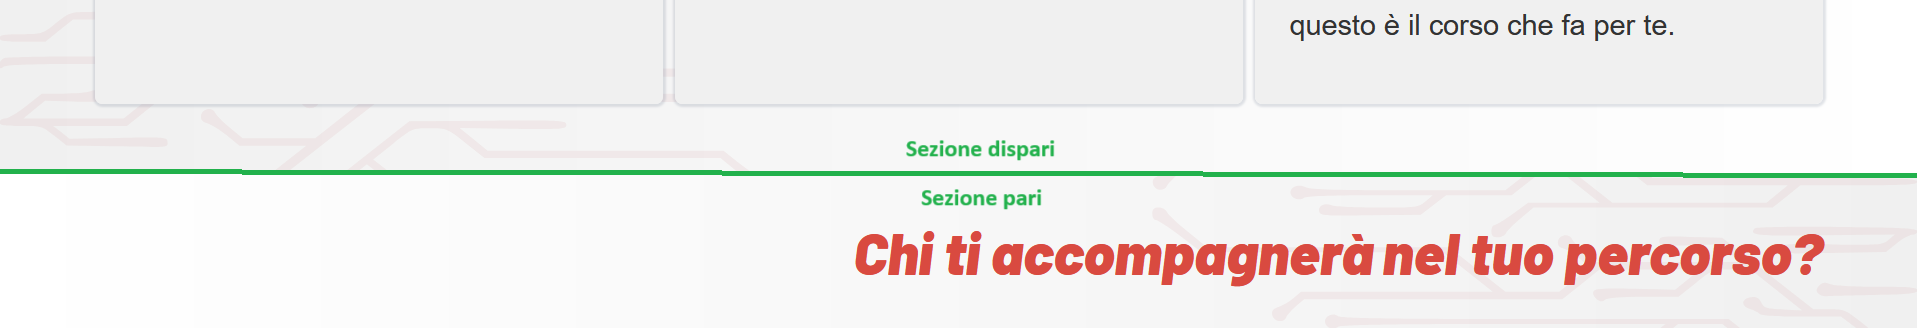
\includegraphics[width=0.95\columnwidth]{applicazione/sfondo_sezioni.png}
    \caption{Esempio di cambio sfondo tra sezioni}
    \label{fig:app_sfondo_sezione}
\end{figure}

Per quanto riguarda la composizione interna delle sezioni dell'infografica, queste sono contenitori \emph{flex} a direzione verticale e comprendono un titolo (\texttt{<h2>}), un sottotitolo (\texttt{<h3>}) e una parte di 
contenuto principale (\texttt{<div>}). Se sono presenti informazioni di corredo, come le opinioni degli studenti sui vari temi, queste sono incluse in ulteriori \texttt{<div>} di appendice.

All'interno dei \texttt{<div>} di contenuto principale, si trovano solitamente i grafici principali e/o i contenitori del testo informativo. Le appendici, invece, contengono i grafici di corredo più piccoli. 

In generale, tutti i grafici sono racchiusi in \texttt{<div>} con attributo \\ \texttt{class="dataviz-wrapper"}, ad eccezione della mappa dei luoghi, che è gestita a sé da un contenitore dedicato. 
Tale struttura consente di creare simultaneamente gli \gls{svg} per i grafici di \gls{datavizg} che hanno la stessa dimensione. 
Nello specifico, si avranno \gls{svg} per i grafici principali di grandi dimensioni, mentre per le appendici si avrà altezza minore. Nel caso siano presenti più grafici affiancati, le dimensioni degli \gls{svg} sono ridotte 
anche per larghezza.
Si riporta di seguito il codice utilizzato per tale obiettivo.
\begin{lstlisting}[style=htmlcssjs]
d3.selectAll(".section-content > .dataviz-wrapper")
    .append("svg")
        .attr("preserveAspectRatio", "xMinYMin meet")
        .attr("viewBox", `0 0 ${widthBig} ${heightBig}`);

d3.selectAll(".section-appendix > .dataviz-wrapper")
    .append("svg")
        .attr("preserveAspectRatio", "xMinYMin meet")
        .attr("viewBox", `0 0 ${widthBig+margin} ${heightSmall+margin}`);

d3.selectAll(".section-content-gridlike > .dataviz-wrapper")
    .append("svg")
        .attr("preserveAspectRatio", "xMinYMin meet")
        .attr("viewBox", `0 0 ${widthSmall+margin} ${heightSmall+margin}`);
\end{lstlisting}
La creazione dei grafici in sè viene poi effettuata selezionando tali \gls{svg} a partire dall'\emph{id} della sezione di riferimento. 

Questo approccio consente dunque una facile aggiunta e creazione dinamica degli \gls{svg}, che sia coerente con il resto dell'infografica
e che non comporti ripetizioni inutili di codice.

\paragraph{Elementi interattivi non specifici.}
Sono presenti alcuni elementi interattivi ricorrenti in più parti dell'infografica, quali:
\begin{itemize}
    \item \textbf{Tooltip su testo}, usati per spiegare e/o approfondire alcune parti del testo. Tali \emph{tooltip}
    sono visibili quando l'utente passa il cursore su parti specifiche indicate da una ``i'' cerchiata.
    \begin{figure}[h]
        \centering
        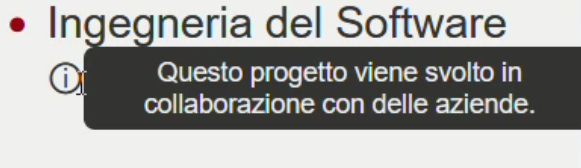
\includegraphics[width=0.3\columnwidth]{applicazione/i-tooltip.png}
        \caption{Esempio di tooltip su testo}
        \label{fig:app_i-tooltip}
    \end{figure}
    \\Tale funzionalità è implementata tramite una combinazione di \gls{js} e \gls{css}.
    \item \textbf{Tooltip su grafici}, usati per dettagli aggiuntivi sui dati quando l'utente passa il cursore sui grafici. 
    Questi \emph{tooltip} sono utili per comprendere meglio le informazioni visualizzate, visionando il valore esatto dei dati.
    \begin{figure}[h]
        \centering
        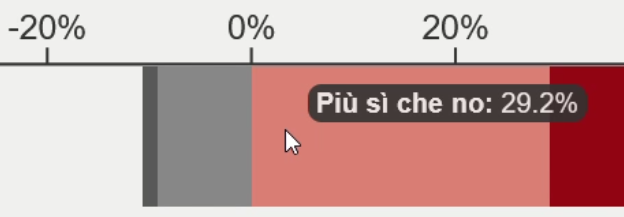
\includegraphics[width=0.3\columnwidth]{applicazione/tooltip.png}
        \caption{Esempio di tooltip su un grafico}
        \label{fig:app_tooltip}
    \end{figure}
    \\Tale funzionalità è implementata tramite una combinazione di \gls{js} e \gls{css}, utilizzando anche \gls{d3g} per la selezione dell'elemento del grafico in questione.
    \item \textbf{Contenitori collassabili}, usati per contenere i grafici rappresentanti le opinioni degli studenti sui vari temi. Questi contenitori 
    possono essere aperti o chiusi tramite apposito pulsante (+ o -), consentendo di visualizzare o nascondere rapidamente queste informazioni extra.
    Questa funzionalità è particolarmente utile in un'infografica \emph{densa} e lunga come la presente, in quanto permette di rendere la navigazione più fluida e 
    migliorare così esperienza utente.
    \begin{figure}[h]
        \centering
        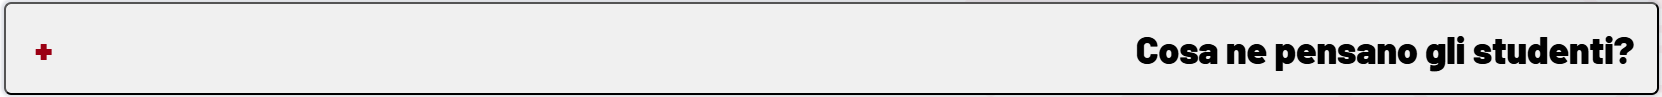
\includegraphics[width=0.8\columnwidth]{applicazione/accordion.png}
        \caption{Esempio di contenitore ``collassato''}
        \label{fig:app_accordion}
    \end{figure}
    \\Tale funzionalità è implementata tramite una combinazione di \gls{js} e \gls{css}.
    \item \textbf{\emph{Panning} e zoom}, utilizzati per esplorare i grafici principali di ogni sezione. Essi permettono agli utenti di ingrandire e spostare la visualizzazione 
    per esaminare dettagli specifici oppure per adattare la visualizzazione su schermi di dimensioni più ridotte. 
    
    Tali funzionalità sono implementate attraverso \gls{d3g} e, in particolare, tramite \texttt{d3.zoom()}.
    \item \textbf{Scorrimento orizzontale}, utilizzato per esplorare i grafici di corredo, che hanno un'ampia larghezza e un'altezza non elevata. È necessaria tale funzionalità per poter vedere questi 
    grafici in dispostivi con schermi piccoli, specie se sviluppati verticalmente come gli smartphone. 
    
    Tale funzionalità è implementata tramite una regola \gls{css} e, in particolare, ponendo \texttt{overflow: auto;}.
\end{itemize}
Un altro elemento interattivo, non associabile a nessuna sezione specifica, è il pulsante che consente di aprire il \emph{chatbot}.
\begin{figure}[H]
    \centering
    
\includegraphics[width=0.1\columnwidth]{applicazione/chat-button.png}
    \caption{Pulsante per l'apertura del chatbot.}
    \label{fig:app_chatbot-button}
\end{figure}
\noindent Questo pulsante si trova in posizione ``galleggiante'' nell'angolo in basso a destra dell'infografica. Tuttavia, è possibile anche spostare tale 
pulsante, trascinandolo a piacimento all'interno della schermata. Ciò consente di accedere facilmente alla chat in qualsiasi momento e, al contempo, evitare che 
questo pulsante copra parti importanti del contenuto.

\subsubsection{Struttura dell'infografica per sezione}
Si riportano di seguito le varie sezioni dell'infografica.

Si segnala che lo sfondo utilizzato nelle sezioni del contenuto principale non è visibile nelle figure qui presentate a causa della strumentazione utilizzata per la loro generazione. 
Si prega, dunque, di fare riferimento alla figura \ref{fig:app_sfondo_sezione} per visualizzarne i dettagli.

\paragraph{Introduzione.} La sezione introduttiva dell'infografica è illustrata nella figura seguente \ref{fig:app_intro}.
\begin{figure}[H] 
    \centering 
    
\includegraphics[width=\columnwidth]{applicazione/intro.png} 
    \caption{Sezione introduttiva dell'infografica}
    \label{fig:app_intro}
\end{figure}
L'elemento principale di tale sezione è il titolo, inserito in un tag \texttt{<h1>} e caratterizzato da dimensioni molto elevate che scalano 
in base alle dimensioni del dispositivo, mantenendo però il forte impatto visivo.
La sezione in sé, grazie a specifiche regole \gls{css}, ricopre l'intero schermo, andando così a rafforzare ancora di più l'impatto visivo. 

Si è inoltre deciso di utilizzare uno sfondo rosso per questa sezione che, non solo amplifica l'attenzione sul titolo, ma anche la differenzia
visivamente dal resto del flusso informativo, rispondendo così alle esigenze progettuali.
 
In aggiunta, sono stati inseriti i loghi dell'Università e del dipartimento del corso per conferire autorità e contestualizzare il corso stesso. 
Tuttavia, questi loghi sono stati posizionati in secondo piano o marginalmente, poiché l'obiettivo principale è valorizzare il corso in sé per le sue caratteristiche e opportunità, 
piuttosto che per l'affiliazione con l'Università stessa.

\paragraph{Requisiti.} La sezione riguardante i requisiti di accesso al corso è illustrata nella figura seguente \ref{fig:requisiti}.
\begin{figure}[H] 
    \centering 
    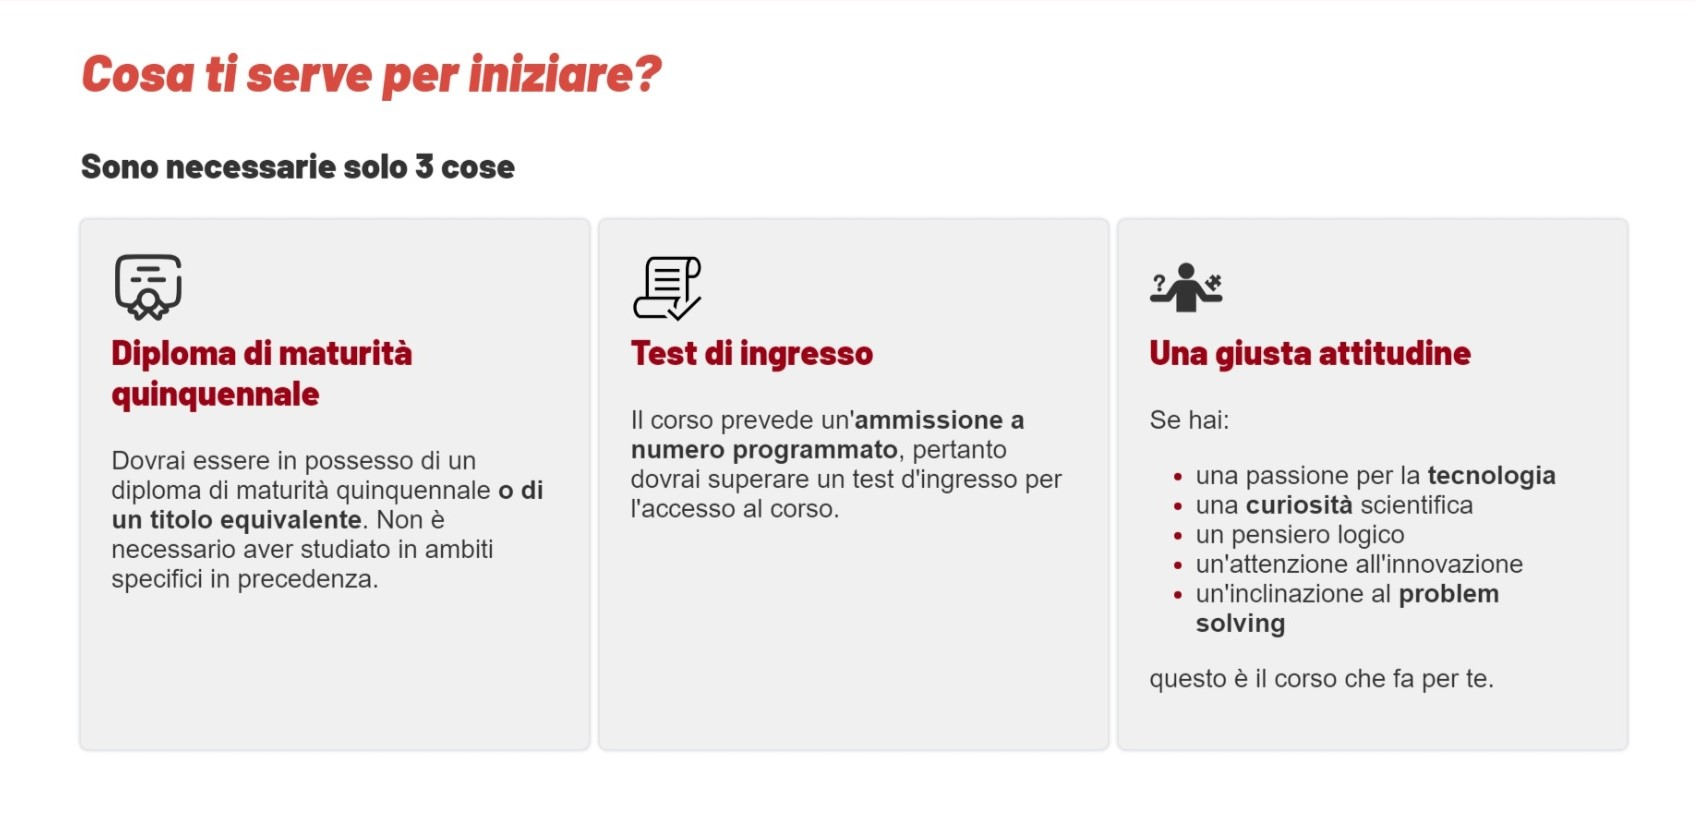
\includegraphics[width=\columnwidth]{applicazione/requisiti.jpeg} 
    \caption{Sezione dell'infografica sui requisiti del corso}
    \label{fig:requisiti}
\end{figure}
\noindent Si ha semplicemente un \texttt{<div>} con \emph{layout} a griglia che contiene e organizza i singoli contenitori dei requisiti.
Tale \emph{layout} è progettato per adattarsi automaticamente alle dimensioni dello schermo, disponendo i requisiti verticalmente su schermi 
più stretti e orizzontalmente su schermi più ampi. Ciò garantisce una leggibilità ottimale e una disposizione 
chiara dei contenuti in tutte le situazioni.

\paragraph{Profilo studenti.} La sezione riguardante il profilo degli studenti è illustrata nella figura seguente. 
\begin{figure}[H] 
    \centering 
    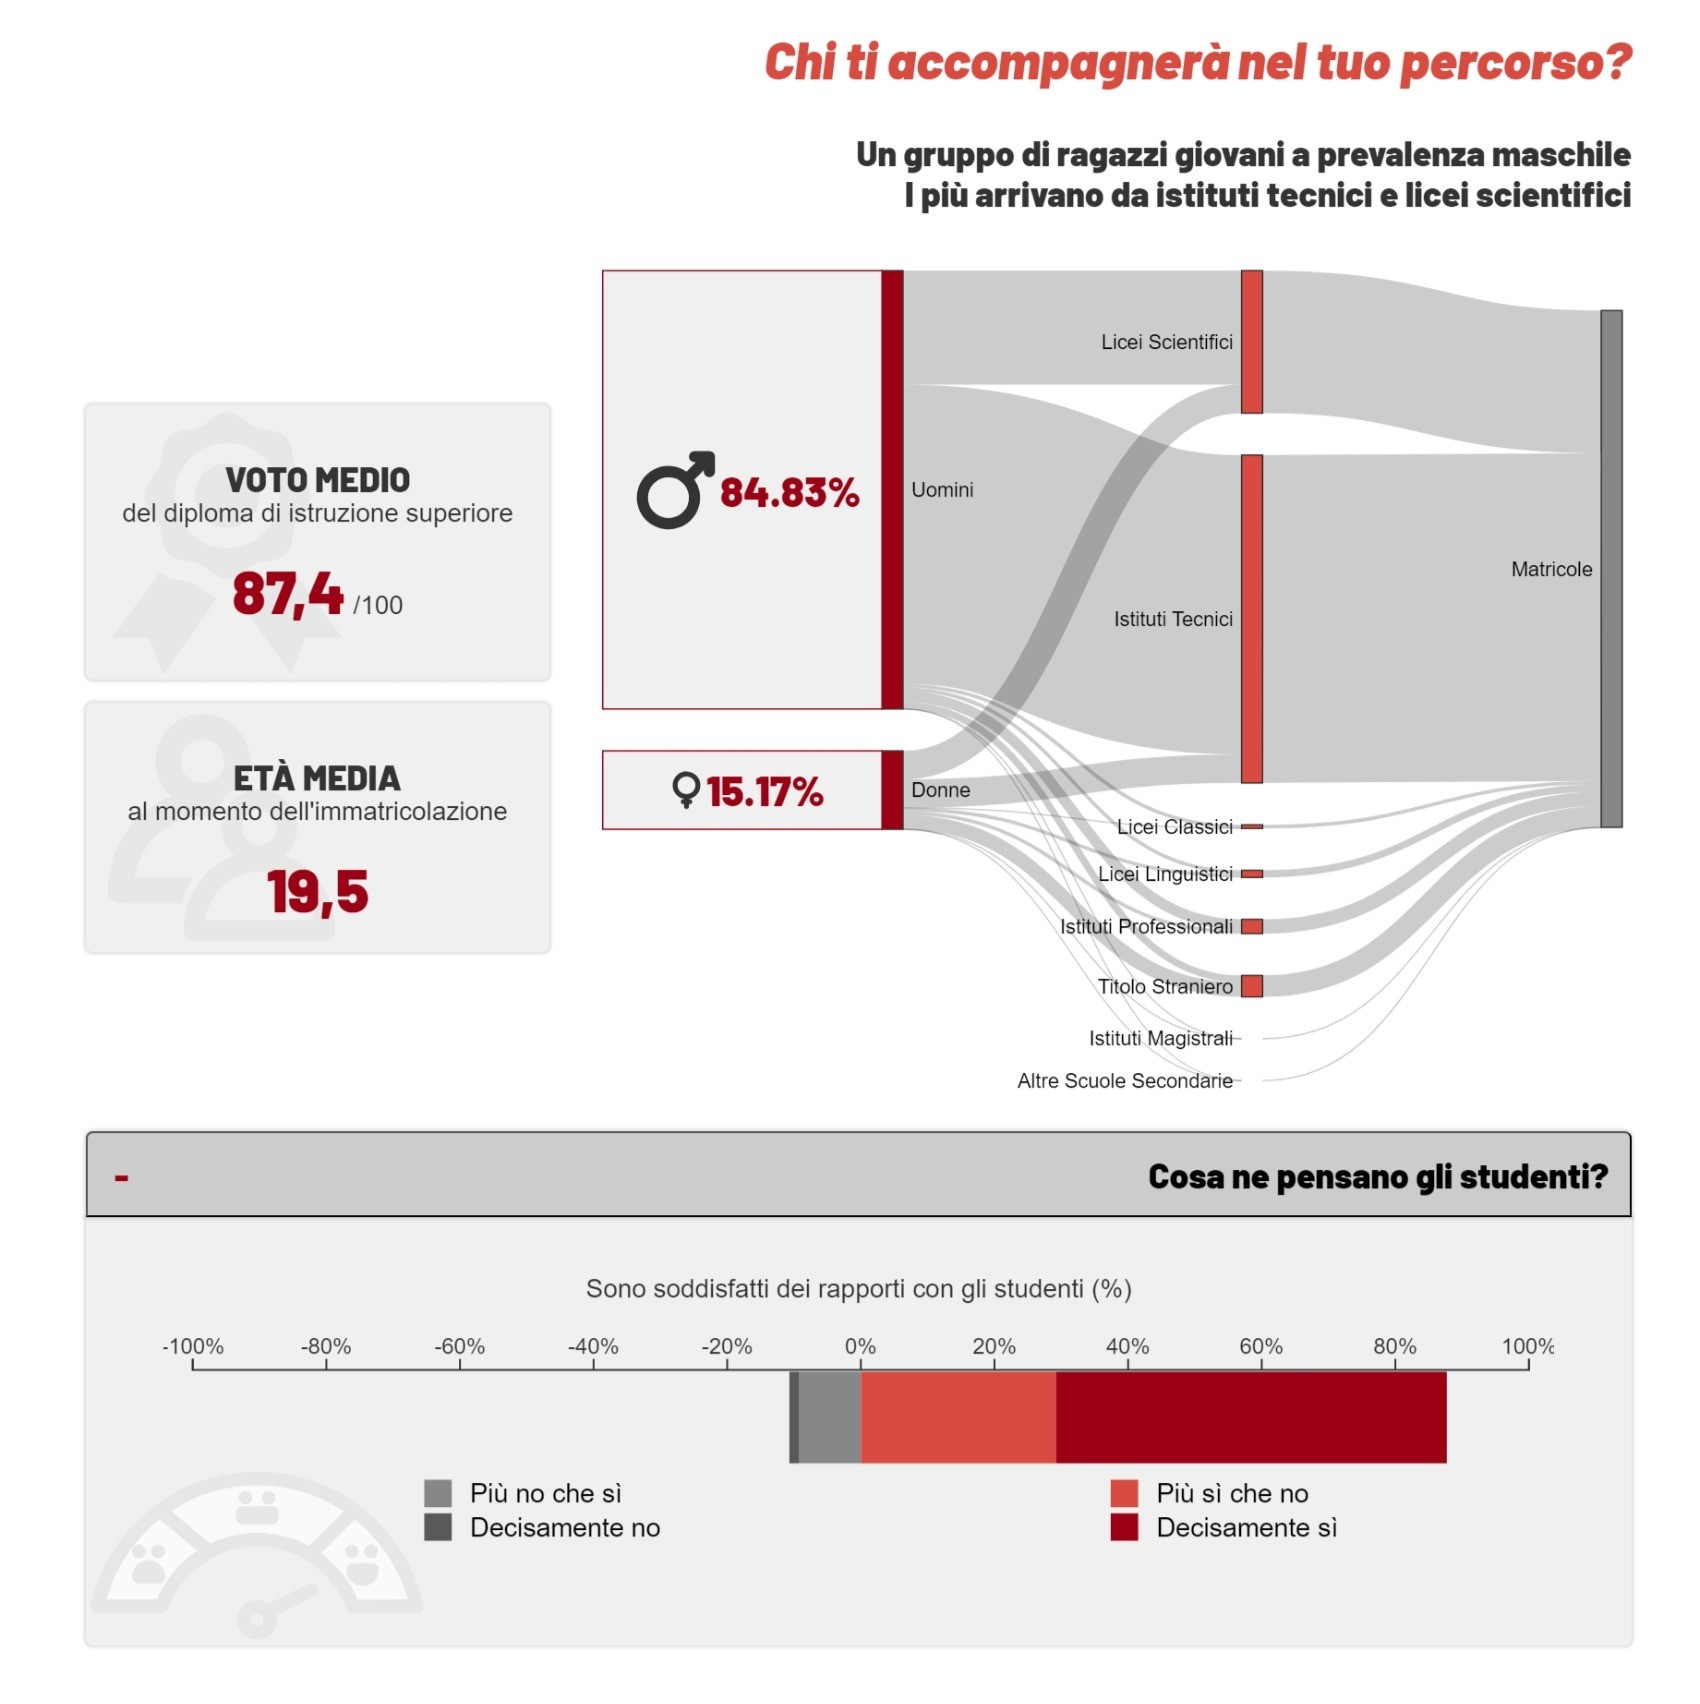
\includegraphics[width=\columnwidth]{applicazione/profilo_studenti.jpeg} 
    \caption{Sezione dell'infografica sul profilo degli studenti}
    \label{fig:app_profilo_stud}
\end{figure}
\noindent Questa sezione fornisce una panoramica del profilo degli studenti, in particolare fornisce informazioni riguardanti il voto e l'età media 
tramite contenitori e dettagli sul sesso e la scuola di provenienza tramite un diagramma di Sankey.

Tale grafico, oltre agli elementi di interazione generale, ne presenta uno ulteriore: posizionando il cursore sui nodi del diagramma si ha un'animazione 
che colora gradualmente i flussi derivanti da tale nodo. Ciò consente di rendere più leggibili ed evidenziare ulteriormente i dati che l'utente sta visionando.
La figura \ref{fig:app_profilo_stud_animated} mostra l'aspetto del diagramma dopo tale animazione.
\begin{figure}[H] 
    \centering 
    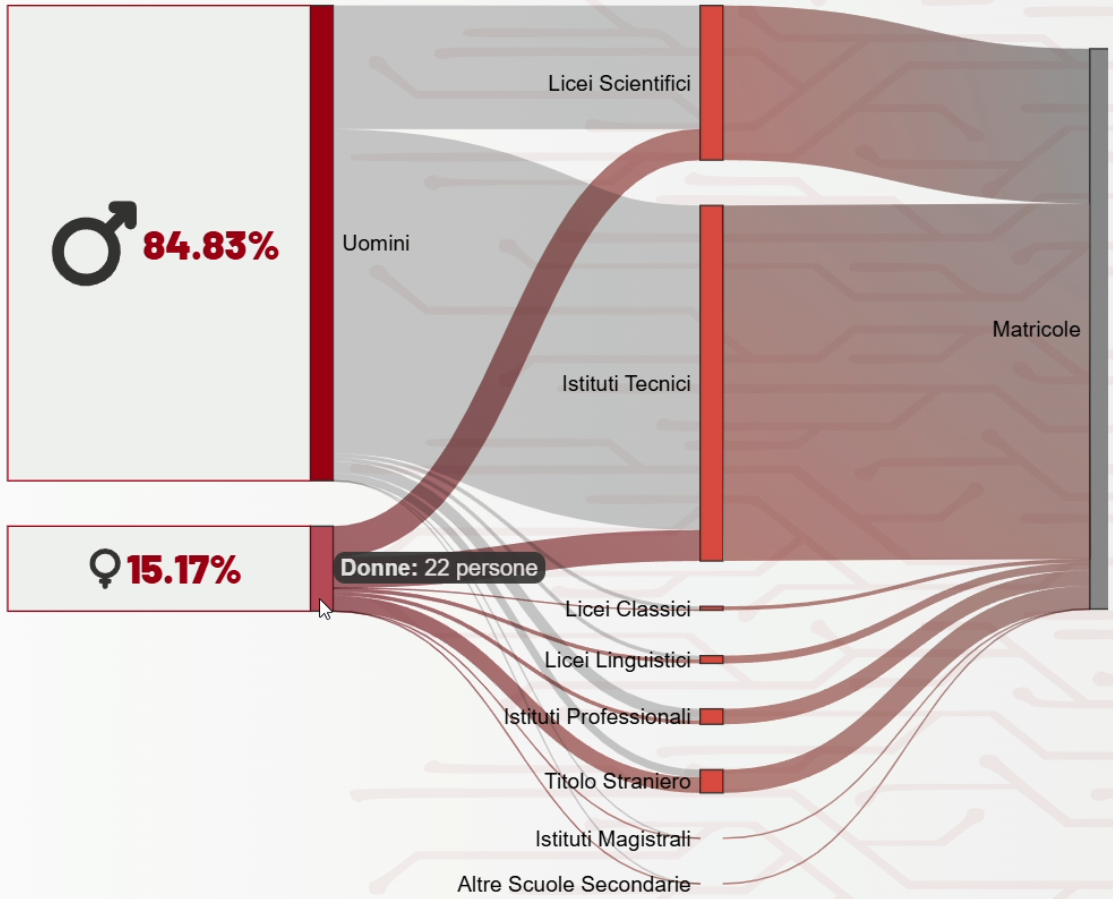
\includegraphics[width=0.6\columnwidth]{applicazione/profilo_studenti_animated.png} 
    \caption{Diagramma di Sankey sul profilo degli studenti animato}
    \label{fig:app_profilo_stud_animated}
\end{figure}

In appendice, su un contenitore collassabile, viene infine riportato un grafico di corredo riguardante l'opinione degli studenti sui rapporti con gli altri studenti.

\bigskip
\noindent Si noti che, anche in questo caso, per garantire la leggibilità della sezione anche per schermi di diverse dimensioni, la parte principale della sezione viene adattata 
in base al dispositivo utilizzato. Nello specifico, per schermi più stretti, i contenitori dei dati e il diagramma di Sankey vengono posti uno sopra l'altro, piuttosto che affiancati.

\paragraph{Luoghi di interesse.} La sezione riguardante le strutture universitarie d'interesse è illustrata nella figura seguente. 
\begin{figure}[H] 
    \centering 
    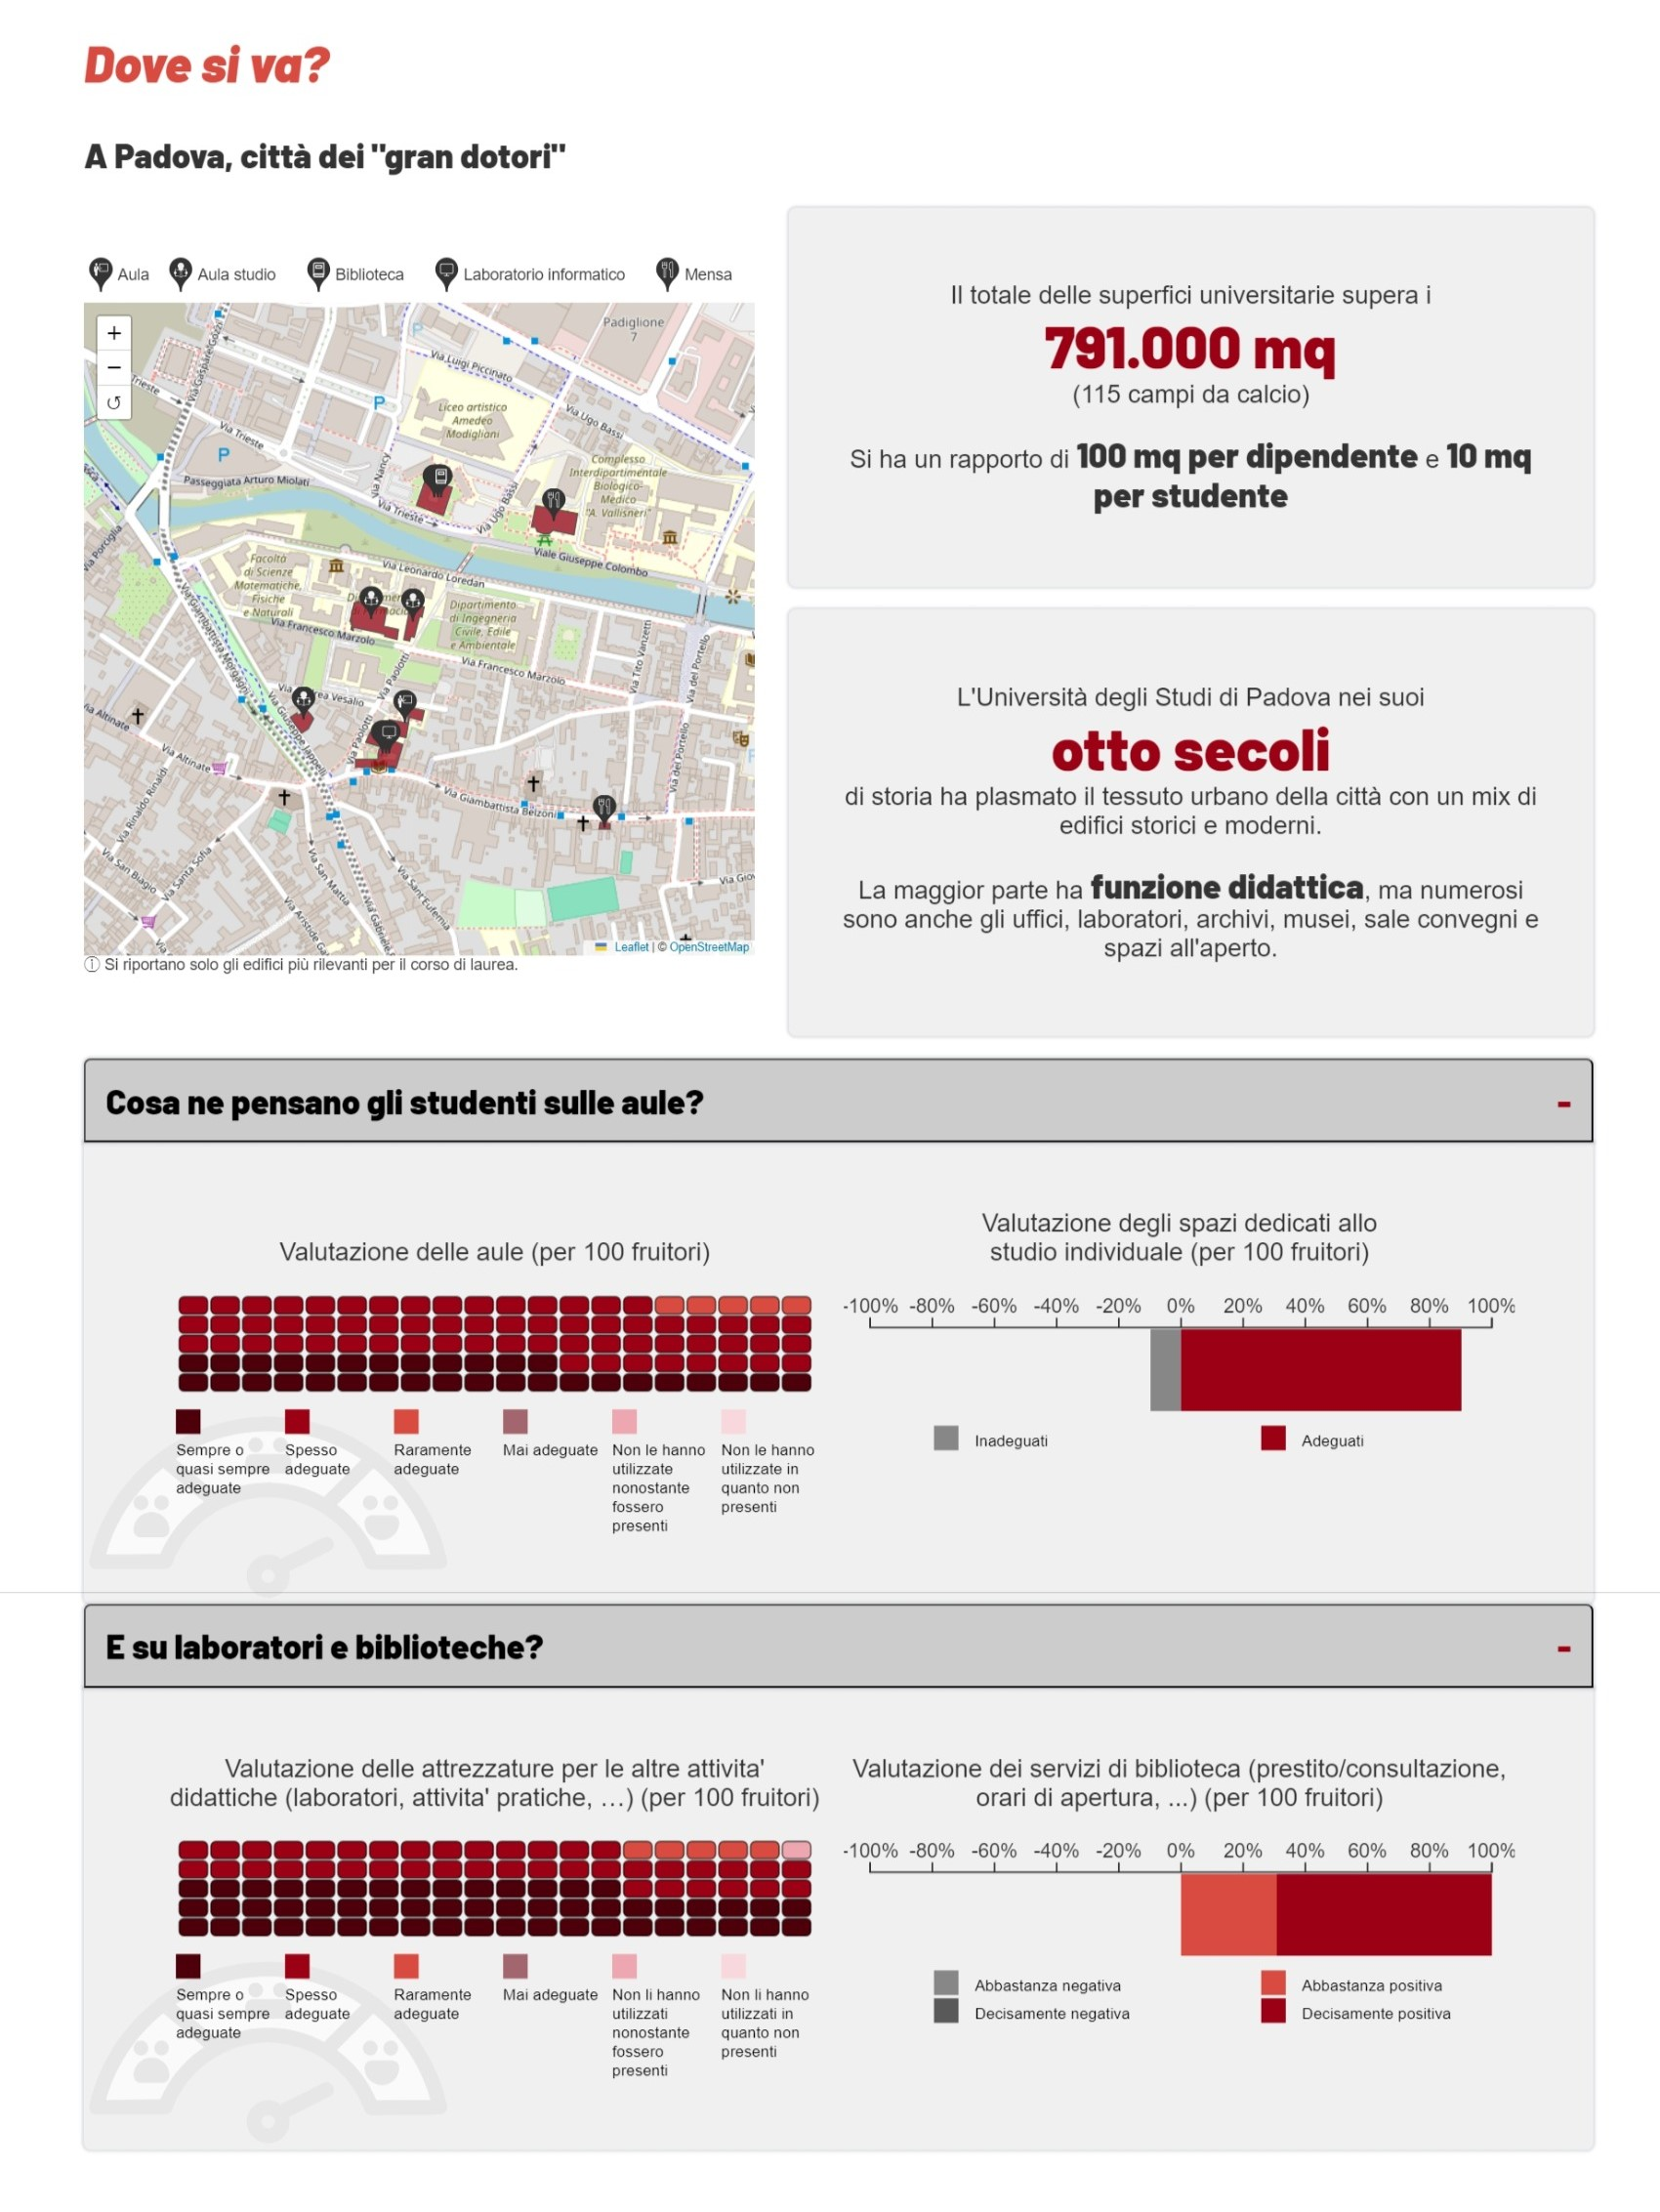
\includegraphics[width=\columnwidth]{applicazione/luoghi.jpeg} 
    \caption{Sezione dell'infografica sui luoghi d'interesse}
    \label{fig:app_luoghi}
\end{figure}
\noindent Questa sezione fornisce una panoramica delle strutture dell'Università che potrebbero essere interessanti per un futuro studente del corso.
In particolare, fornisce informazioni riguardanti le proprietà dell'Università nel loro insieme tramite contenitori e dettagli sulle strutture di interesse 
tramite una mappa. 

In questa mappa, le strutture vengono evidenziate in rosso per metterle in risalto e visualizzarne più velocemente la dimensione.
Inoltre, vengono inserite delle puntine che indicano la tipologia di struttura; la cui legenda è riportata al di sopra della mappa.
Cliccando su tali puntine è possibile vedere i dettagli riguardanti la struttura corrispondente, inclusi nome e tipologia, nonché eventuali altri dettagli utili. 
Inoltre, la struttura viene evidenziata in un altro colore che ne enfatizza ulteriormente la selezione.
Ciò permette di aumentare la leggibilità della mappa e, al contempo, di fornire ulteriori informazioni.
Se una stessa struttura ha tipologia mista, ovvero ha più usi, vengono poste più puntine sovrapposte. Tuttavia, è possibile vedere individualmente ciascuna puntina 
cliccando sull'insieme di queste.
La figura \ref{fig:app_mappa_interazione} mostra l'interazione.
\begin{figure}[H] 
    \centering 
    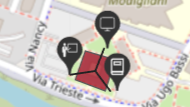
\includegraphics[width=0.3\columnwidth]{applicazione/mappa_spiderfier.png} 
    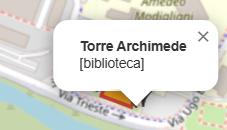
\includegraphics[width=0.3\columnwidth]{applicazione/mappa_popup.png} 
    \caption{Mappa dei luoghi dell'Università - visualizzazione individuale delle puntine e popup}
    \label{fig:app_mappa_interazione}
\end{figure}

In appendice, su un contenitore collassabile, vengono riportati diversi grafici di corredo riguardanti l'opinione degli studenti sui vari tipi di strutture.

\bigskip
\noindent Si noti che, anche in questo caso, per garantire la leggibilità della sezione anche per schermi di diverse dimensioni, la parte principale della sezione viene adattata 
in base al dispositivo utilizzato. Nello specifico, per schermi più stretti, i contenitori dei dati e la mappa vengono posti uno sopra l'altro, piuttosto che affiancati.

\paragraph{Materie di studio.} La sezione riguardante le materie di studio è illustrata nella figura seguente. 
\begin{figure}[H] 
    \centering 
    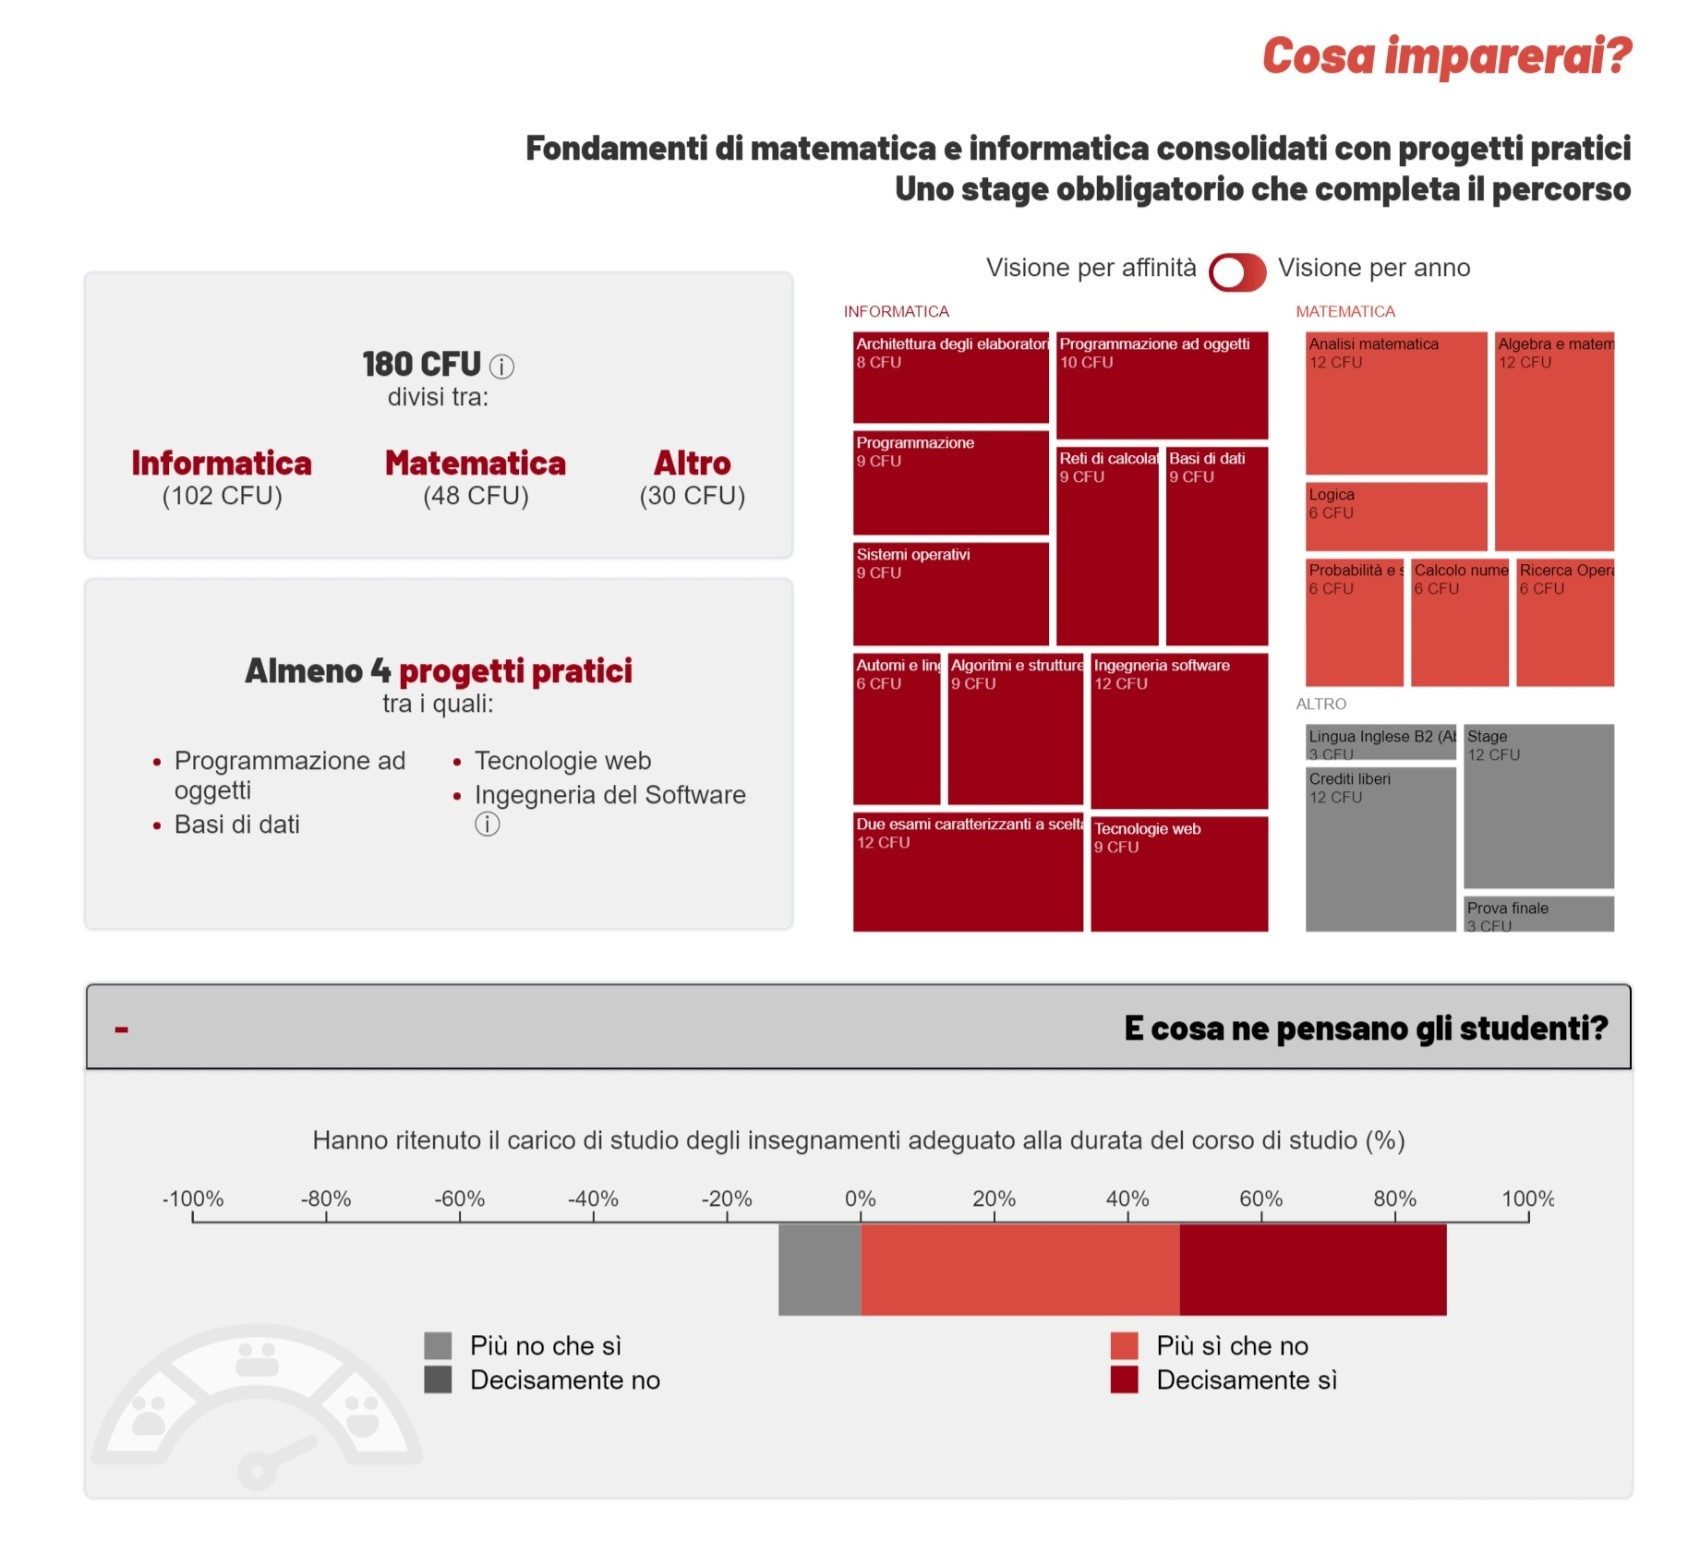
\includegraphics[width=\columnwidth]{applicazione/materie.jpeg} 
    \caption{Sezione dell'infografica sulle materie di studio}
    \label{fig:app_materie}
\end{figure}
\noindent Questa sezione fornisce una panoramica delle materie del corso. In particolare, fornisce delle informazioni riguardanti i progetti pratici e una quantificazione generale di impegno 
tramite contenitori, mentre utilizza un \emph{Treemap} per visualizzare le materie specifiche e il loro peso sul corso.

Tale grafico consente una visualizzazione sia per affinità con temi matematici, informatici o altro, sia per anno di offerta.
Tale configurazione è possibile grazie ad uno \emph{switch} posto al di sopra del grafico.

\bigskip
\noindent Si noti che, anche in questo caso, per garantire la leggibilità della sezione anche per schermi di diverse dimensioni, la parte principale della sezione viene adattata 
in base al dispositivo utilizzato. Nello specifico, per schermi più stretti, i contenitori dei dati e il \emph{treemap} vengono posti uno sopra l'altro, piuttosto che affiancati.

\paragraph{Regolarità negli studi ed esiti.} La sezione riguardante il percorso universitario degli studenti (per durata e voto) è illustrata nella figura seguente. 
\begin{figure}[H] 
    \centering 
    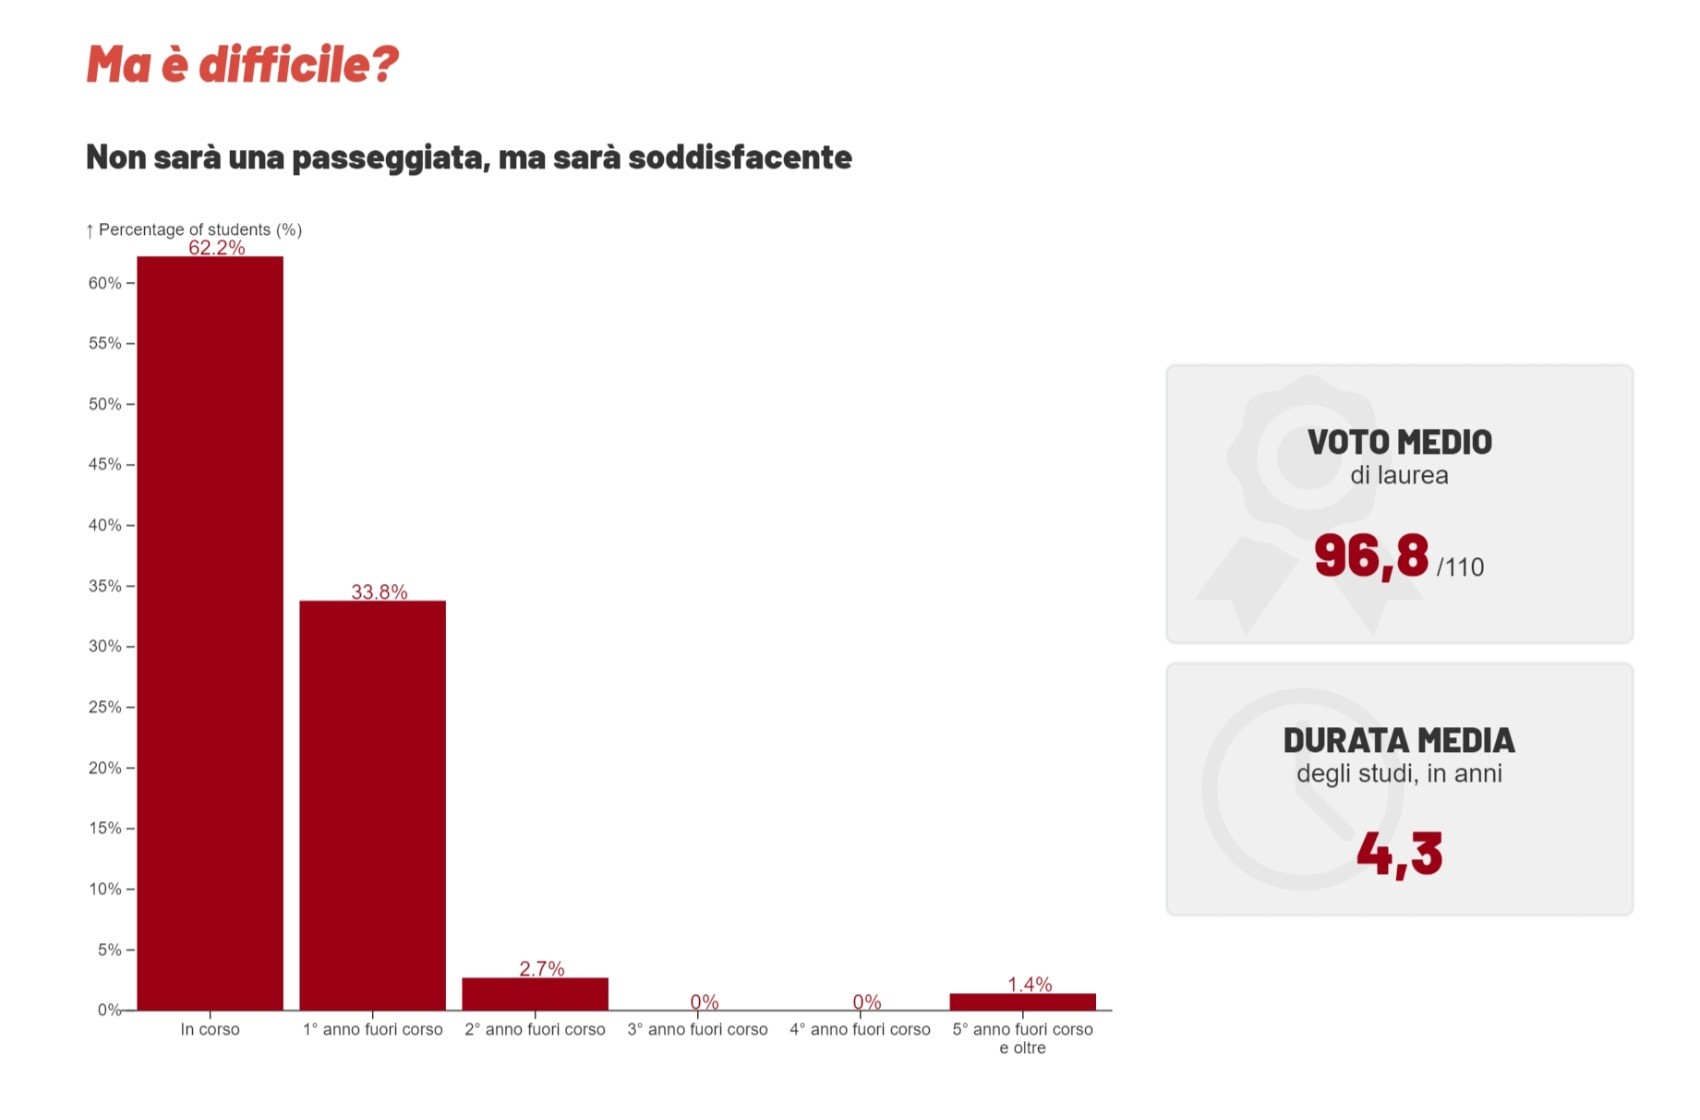
\includegraphics[width=\columnwidth]{applicazione/durata.jpeg} 
    \caption{Sezione dell'infografica sul percorso universitario per durata e voto}
    \label{fig:app_durata}
\end{figure}
\noindent Questa sezione presenta in maniera molto semplice la riuscita e regolarità del percorso di studio degli studenti. In particolare, si utilizza un grafico a barre 
per rappresentare la durata del percorso, mostrando le quantità di studenti in corso e fuori corso; mentre, si utilizzano dei contenitori per mostrare le statistiche medie relative 
a voto e durata complessiva.

\bigskip
\noindent Si noti che, anche in questo caso, per garantire la leggibilità della sezione anche per schermi di diverse dimensioni, la parte principale della sezione viene adattata 
in base al dispositivo utilizzato. Nello specifico, per schermi più stretti, i contenitori dei dati e il grafico vengono posti uno sopra l'altro, piuttosto che affiancati.

\paragraph{Opportunità post-laurea.} La sezione riguardante i percorsi intrapresi post-laurea (lavorativi o formativi) è illustrata nella figura seguente. 
\begin{figure}[H] 
    \centering 
    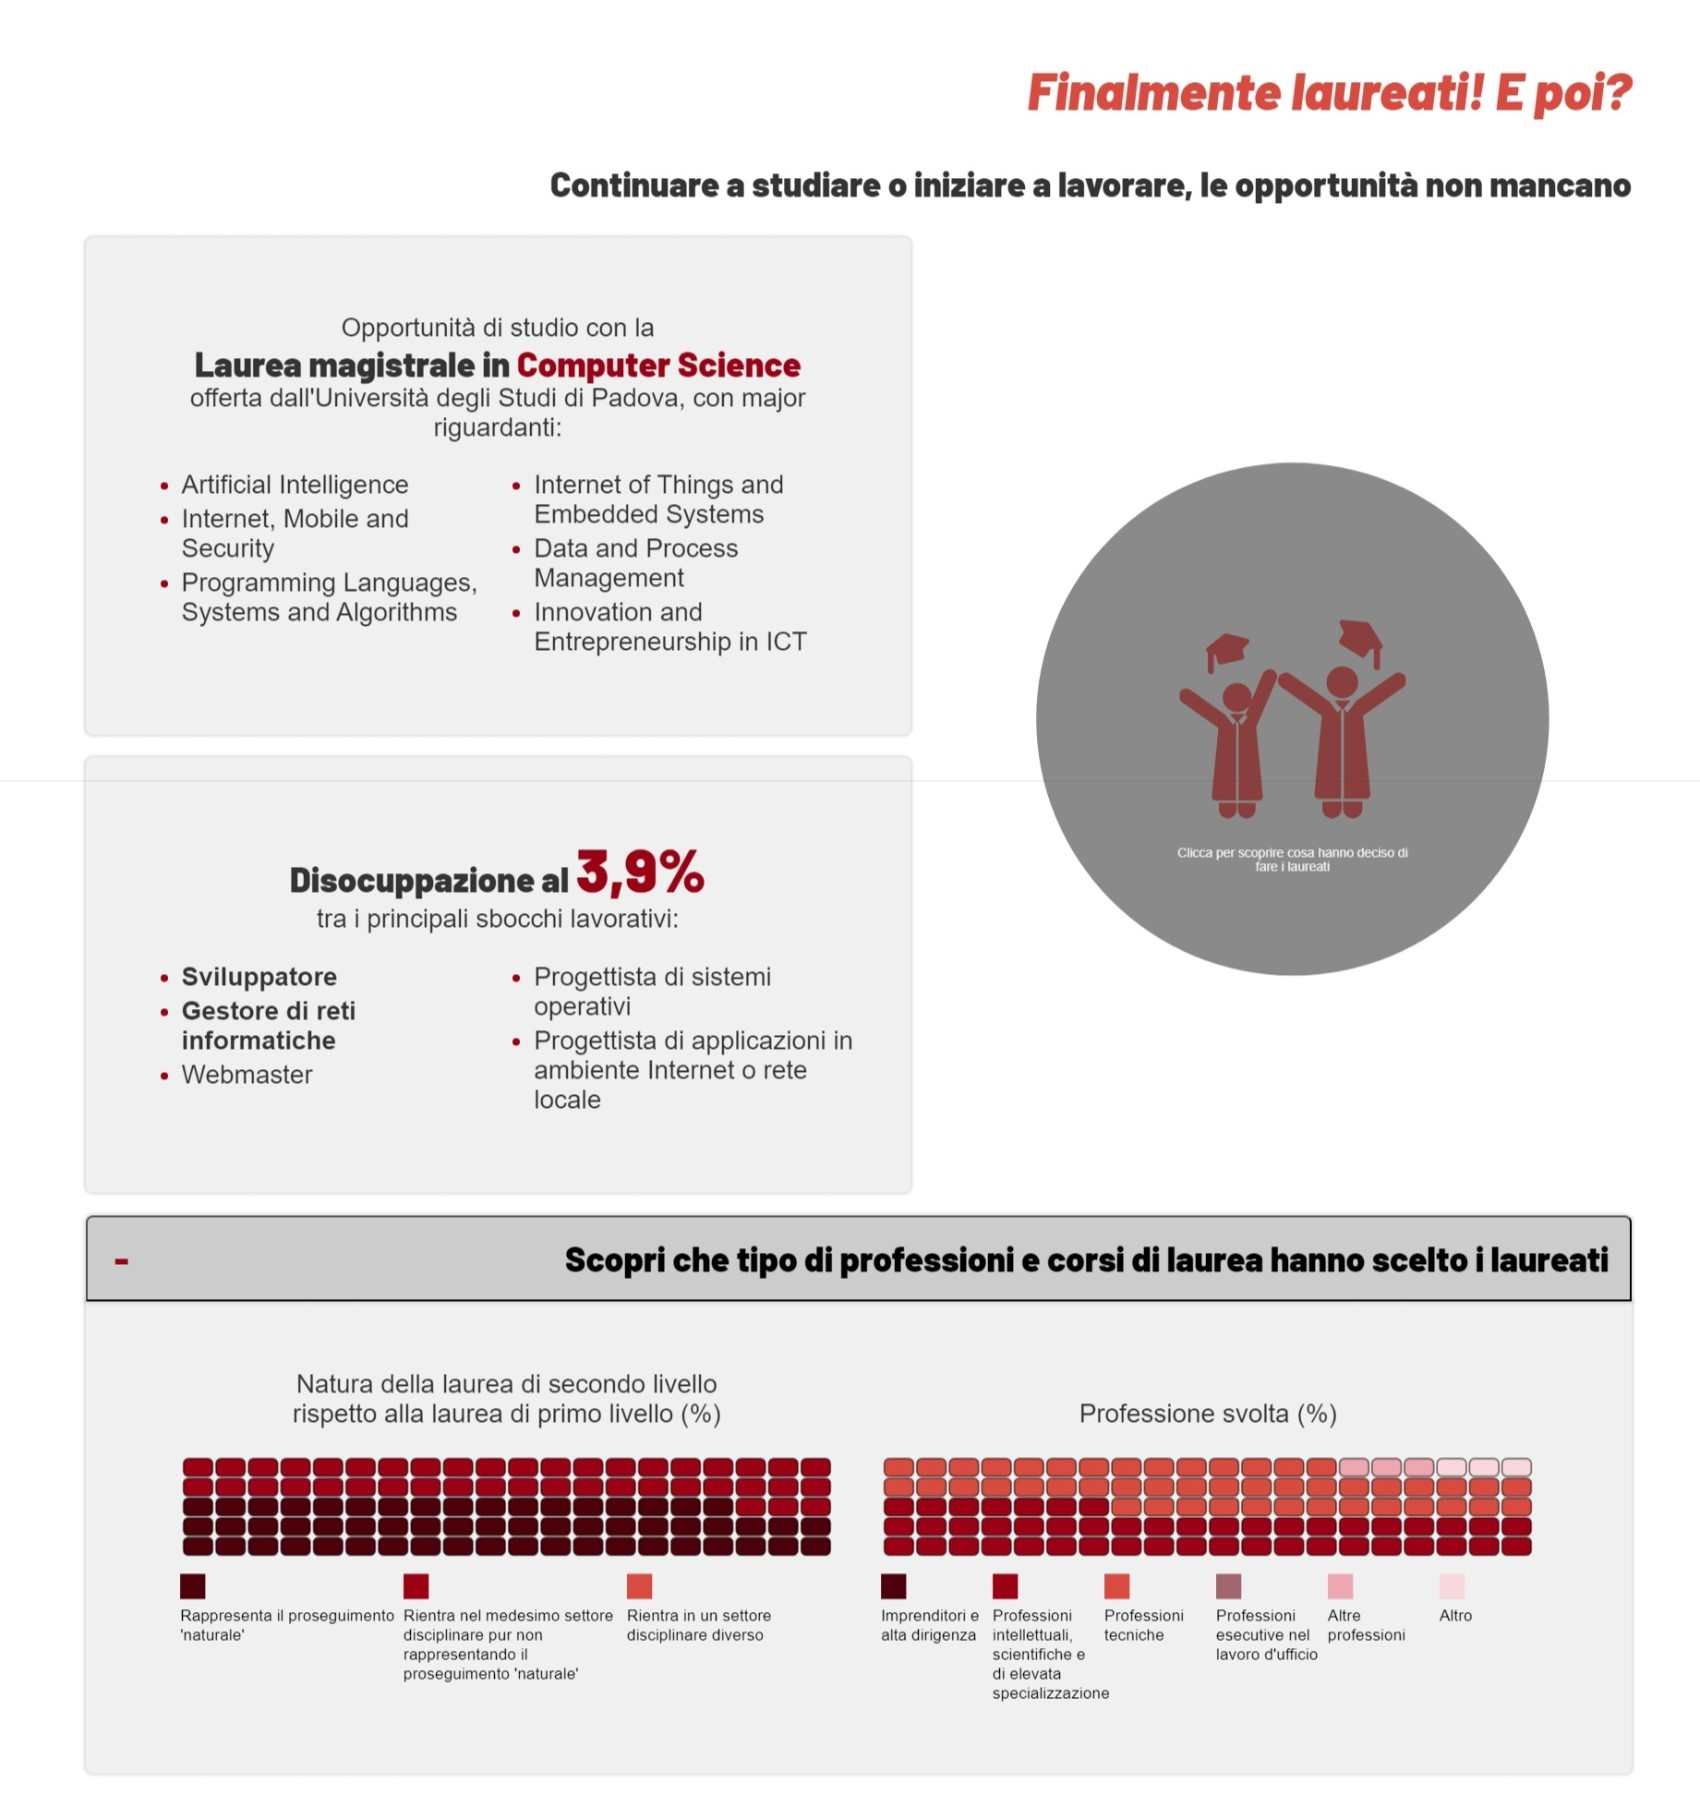
\includegraphics[width=\columnwidth]{applicazione/post-laurea.jpeg} 
    \caption{Sezione dell'infografica riguardante i percorsi intrapresi post-laurea}
    \label{fig:app_post-laurea}
\end{figure}
\noindent Questa sezione presenta una panoramica delle possibilità per gli studenti dopo la laurea. In particolare, si utilizza un diagramma di Venn per visualizzare la 
proporzione tra studenti e lavoratori. 
Si noti che tale statistica non è mostrata fin da subito, infatti, il diagramma mostra inizialmente solo un cerchio con un'icona di due laureati festeggianti.
Questa scelta è volta ad attirare l'attenzione dell'utente e fare appello alle sue emozioni, creando una visualizzazione più coinvolgente e accattivante. 
Le proporzioni sono visibili semplicemente cliccando sul cerchio stesso, ottenendo un diagramma di Venn proporzionale come illustrato nella figura 
\ref{fig:app_post-laurea_animated}. 

Oltre a tale grafico, sono presenti dei contenitori che descrivono i possibili percorsi, lavorativi o formativi, che i laureati possono intraprendere.
\begin{figure}[H] 
    \centering 
    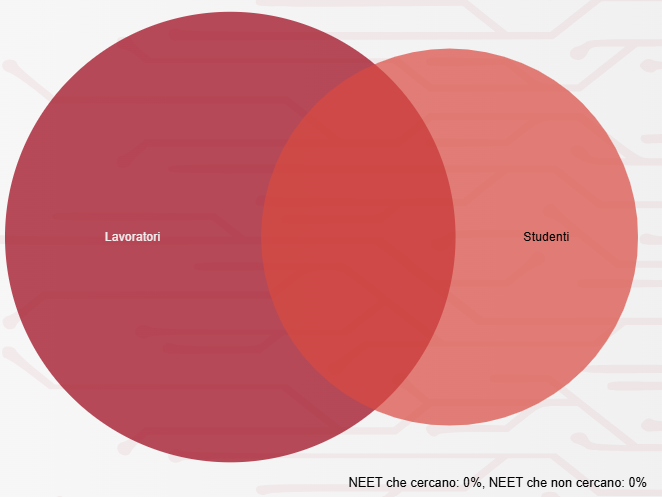
\includegraphics[width=0.6\columnwidth]{applicazione/post-laurea_animated.png} 
    \caption{Diagramma di Venn sulla proporzione di studenti e lavoratori dopo l'animazione}
    \label{fig:app_post-laurea_animated}
\end{figure}

In appendice, su un contenitore collassabile, vengono infine riportati diversi grafici di corredo riguardanti cosa effettivamente hanno scelto di fare gli studenti in caso 
di proseguimento con gli studi e/o lavoro.

\bigskip
\noindent Si noti che, anche in questo caso, per garantire la leggibilità della sezione anche per schermi di diverse dimensioni, la parte principale della sezione viene adattata 
in base al dispositivo utilizzato. Nello specifico, per schermi più stretti, i contenitori dei dati e il diagramma di Venn vengono posti uno sopra l'altro, piuttosto che affiancati.

\paragraph{Opinioni finali.} La sezione riguardante l'opinione sul corso dei laureati è illustrata nella figura seguente. 
\begin{figure}[H] 
    \centering 
    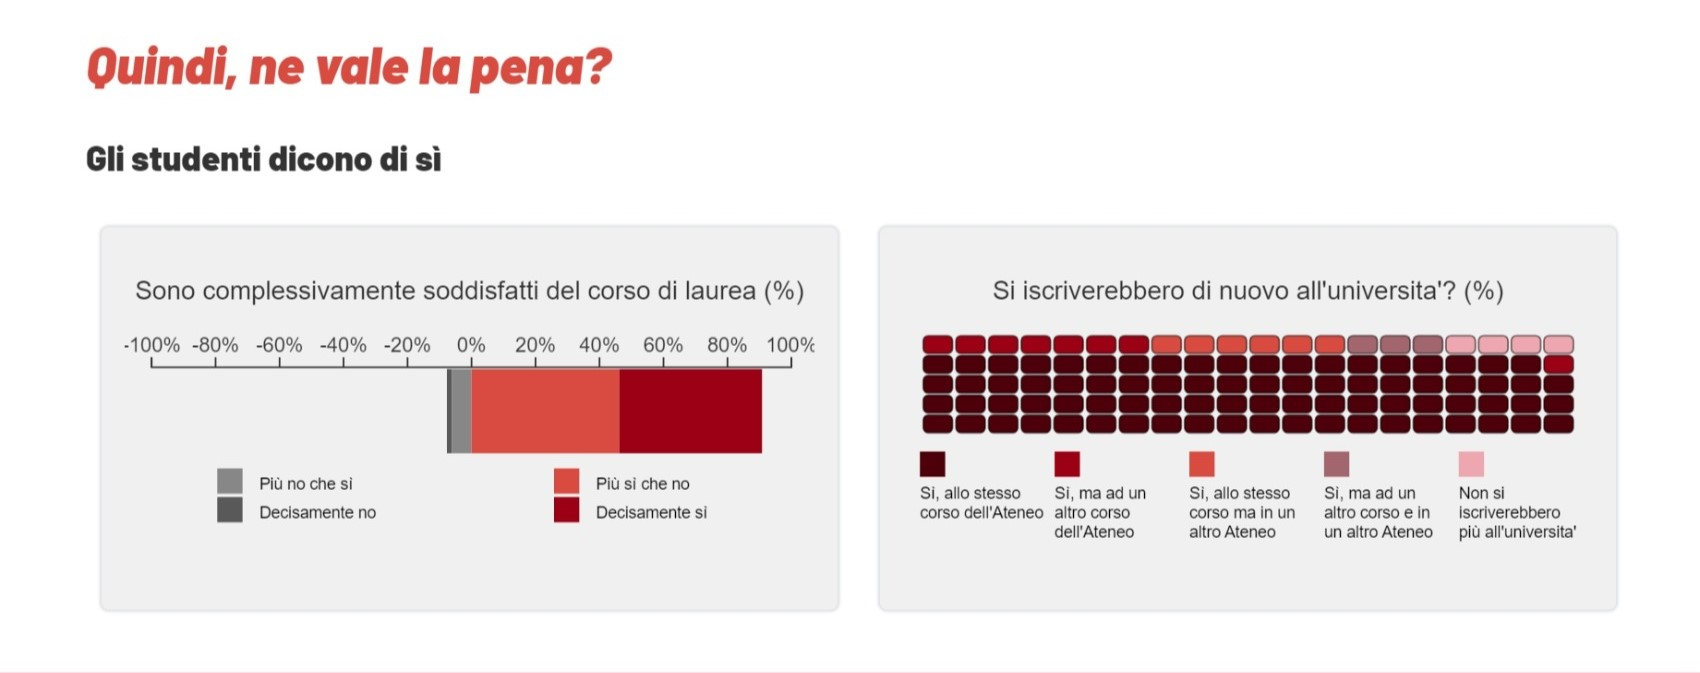
\includegraphics[width=\columnwidth]{applicazione/opinioni_finali.jpeg} 
    \caption{Sezione dell'infografica sull'opinione finale dei laureati}
    \label{fig:opinioni_finali}
\end{figure}
Questa sezione presenta in maniera molto semplice le opinioni finali degli studenti sul corso. In particolare, si utilizzano due grafici rispettivamente per visualizzare la soddisfazione 
generale dei laureati e per indicare se, alla luce della loro esperienza, quest'ultimi sceglierebbero di iscriversi nuovamente al corso.

\bigskip
\noindent Si noti che, anche in questo caso, per garantire la leggibilità della sezione anche per schermi di diverse dimensioni, la sezione viene adattata 
in base al dispositivo utilizzato. Nello specifico, per schermi più stretti, i contenitori dei grafici disposti verticalmente, piuttosto che orizzontalmente

\paragraph{Fonti.} Le note a piè di pagina, contenti le fonti, sono illustrate nella figura seguente. 
\begin{figure}[H] 
    \centering 
    
\includegraphics[width=\columnwidth]{applicazione/fonti.png} 
    \caption{Sezione dell'infografica sulle fonti}
    \label{fig:app_fonti}
\end{figure}
Tale sezione utilizza uno sfondo rosso per segnalarne la distinzione dal normale flusso informativo dell'infografica, similmente a quanto accade per la sezione introduttiva. 
I link alle fonti sono riportati in giallo per differenziarli dal testo normale e, al contempo, garantirne la leggibilità rispetto al colore di sfondo.

\subsubsection{Chatbot}\label{subsubsec:chatbot}
L'infografica dispone di un \emph{chatbot} progettato per rispondere ai dubbi degli utenti e per facilitare la navigazione all'interno dell'infografica, 
essendo essa molto lunga e dunque potenzialmente disorientante.

L'accesso al \emph{chatbot} avviene tramite un pulsante (visibile nella figura \ref{fig:app_chatbot-button}), il quale apre una finestra nell'angolo in basso a destra dell'infografica. 
All'interno di tale finestra gli utenti possono porre domande e ricevere una breve risposta dal \emph{chatbot} per il loro interrogativo. Quest'ultimo, inoltre, rimanda anche alla sezione 
dell'infografica che tratta l'argomento della domanda per avere delle informazioni più dettagliate.
\begin{figure}[H] 
    \centering 
    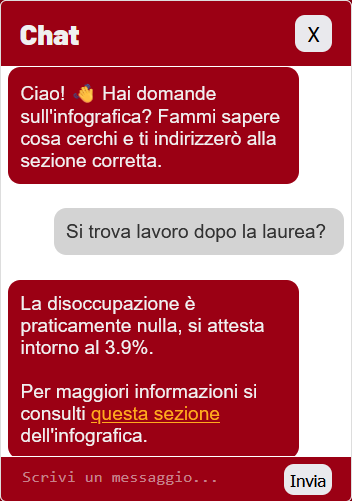
\includegraphics[width=0.35\columnwidth]{applicazione/chat.png} 
    \caption{Esempio di finestra della chat}
    \label{fig:app_chat}
\end{figure}

Dal punto di vista implementativo, gli utenti inseriscono le loro domande in un campo di testo (\texttt{<textarea>}) inserito all'interno di un tag \gls{html} \texttt{<form>}. 
Quando l'utente invia il messaggio, sia tramite pulsante apposito sia tramite ``Invio'' da tastiera, 
viene inviato anche il modulo e, di conseguenza, richiamata una funzione \gls{js} che gestisce le funzionalità della chat.
Nello specifico, tale funzione di occupa di:
\begin{itemize}
    \item Cancellare il contenuto del tag \texttt{<textarea>} e riscriverlo, invece, all'interno dell'area della chat in un nuovo \texttt{<div>} rappresentante il 
    messaggio inviato dall'utente.
    \item Aggiungere un ulteriore \texttt{<div>} all'area di chat che simula una risposta in arrivo dal \emph{bot}. Contiene infatti tre puntini animati a indicare che il messaggio è in fase 
    di elaborazione. L'animazione di tali puntini è realizzata attraverso transizioni \gls{css}.
    \item Richiamare la funzione che genera la risposta al messaggio inviato e inserire tale risposta al posto dei tre puntini.
\end{itemize}
Si noti che la creazione dei messaggi all'interno della chat viene effettuata tramite \gls{d3g}, che consente un inserimento e aggiornamento dinamico degli elementi. 

Per quanto riguarda invece la funzione di generazione della risposta, questa varia in base alla versione dell'infografica utilizzata. Nei paragrafi successivi verranno riportati i dettagli specifici del funzionamento di ciascuna versione.

\paragraph{Generazione della risposta nella versione base.} Viene richiamata la funzione \texttt{answer(q)} passando il messaggio dell'utente come parametro. Tale funzione viene eseguita all'interno di \texttt{setTimeout()} per simulare un'elaborazione 
del messaggio, consentendo anche la visualizzazione dei tre puntini di caricamento anziché mostrare immediatamente la risposta. Ciò consente di fornire l'interazione più naturale e dunque migliorare l'esperienza utente.
\texttt{answer(q)} viene definita come segue:
\begin{lstlisting}[style=htmlcssjs]
function answer(q) {   
    // Remove stop-words of user question
    let filteredUserQ = removeStopWords(q);

    // Remove stop-words from faq questions
    let filteredQs = faq.map(el => 
        removeStopWords(el.question)
    );

    // Stemming of user question
    var stem = PorterStemmerIt.newStemmer('italian').stem;
    filteredUserQ = filteredUserQ.map(el => stem(el));

    // Stemming of faq questions
    filteredQs = filteredQs.map(el => el =
        el.map(item => stem(item))
    );

    // Indexing: for each word in filteredUserQ returns indexes of filteredQs that has that word
    let invertedIndex = Array.from({ length: filteredUserQ.length }, () => []);
    filteredQs.forEach((q, q_index) => {
        filteredUserQ.forEach((word, i_word) => {
            if(q.includes(word)) {
                invertedIndex[i_word].push(q_index);
            }
        })
    });

    const qsIndexes = getQsIndexCorrespondence(invertedIndex);      // sorted array of elements [q_index, terms_count_in_q_index_question]

    if (qsIndexes.length > 0) {
        const highestCorr = faq[parseInt(qsIndexes[0][0])];
        return highestCorr.answer + `<br /><br /> Per maggiori informazioni si consulti <a href="${highestCorr.section}">questa sezione</a> dell'infografica.`;
    }
    else {
        return "Spiacente, non sembra esserci questa informazione nell'infografica. &#128542;";
    }
}
\end{lstlisting}
dove \texttt{faq} è una variabile contenente un array di oggetti nel formato \texttt{[{question: "string", answer: "string", section: "string"}]}, che rappresenta una serie di domande frequenti che l'utente potrebbe fare, 
assieme alle relative risposte e all'\emph{id} della sezione corrispondente nel documento \gls{html}. Tale array è ricavato da un file \gls{jsong} tramite la funzione \texttt{d3.json()} fornita da \gls{d3g}. 
È importante notare che il \emph{chatbot} diventa utilizzabile solo dopo che questo file è stato completamente caricato.

\noindent Per quanto riguarda invece le altre funzioni richiamate, si hanno:
\begin{itemize}
    \item \texttt{removeStopWords(text)}, implementata dallo stagista, che serve a rimuovere le \gls{stopwordsg} dal testo. 
    Tali parole sono rimosse per migliorare l'efficacia della ricerca. A tal fine, il testo viene anche ``normalizzato'', ovvero viene
    tolta la punteggiatura e la stringa viene trasformata tutta in minuscolo.
    Alla fine del processo, \texttt{removeStopWords(text)} restituisce un array contenente le parole rimaste dopo le suddette operazioni.
    \item \texttt{stem(word)}, fornita da una libreria esterna, che serve a effettuare lo \gls{stemmingg} della parola.
    \item \texttt{getQsIndexCorrespondence(indexPerWord)}, implementata dallo stagista, dove \texttt{indexPerWord} è un array in cui ogni elemento rappresenta 
    una parola della frase da confrontare, nel caso specifico una parola della domanda dell'utente. Ciascuno di questi elementi è costituito da un array 
    che contiene gli indici dei documenti - nel caso specifico gli indici delle domande in \texttt{faq} - in cui la suddetta parola è presente.
    La funzione conta quante volte uno stesso indice di documento appare e ordina i risultati in base al numero di occorrenze. Si ottiene dunque, nel caso specifico, 
    un array ordinato del tipo \texttt{[[indice domanda FAQ, numero di occorrenze di parole del messaggio dell'utente nella domanda]]}. 
\end{itemize}
La funzione \texttt{answer(q)} si occupa dunque di:
\begin{itemize}
    \item Rimuovere le \gls{stopwordsg} sia dalla domanda dell'utente che dalle domande frequenti.
    \item Applicare il processo di \gls{stemmingg} sempre a entrambi.
    \item Cercare nelle domande frequenti così ottenute quelle che contengono le parole dell'utente risultanti dalle operazioni sopra.
    \item Contare le occorrenze di queste parole nelle domande e determinare quale domanda ha il maggior numero di corrispondenze.
    \item Ritornare il contenuto della risposta (sotto forma di \gls{html}), comprendente \texttt{answer} di \texttt{faq} relativa 
    alla domanda individuata e un paragrafo aggiuntivo con il collegamento alla sezione dell'infografica relativa (preso da \texttt{section} di \texttt{faq}).
    Nel caso non ci siano corrispondenze in nessuna domanda del \texttt{faq}, viene restituito un messaggio di scuse.
\end{itemize}

\paragraph{Generazione della risposta nella versione integrata.} Innanzitutto, si precisa che, prima di utilizzare questa versione, è necessario aver configurato correttamente il database con il file contenente le informazioni e 
le sezioni. Questo passaggio è fondamentale per assicurare che il sistema possa accedere e recuperare i dati necessari a generare risposte pertinenti.

Per quanto riguarda la generazione della risposta in sé, si effettua una richiesta tramite \texttt{fetch} all'\emph{endpoint} fornito da un server Flask, passando il messaggio dell'utente come corpo della richiesta. 
La risposta al messaggio viene quindi elaborata dal server tramite la funzione \gls{pythong} \texttt{response\_generator} (implementata dal collega Fabio Meneghini) e restituita, poi, in risposta alla richiesta 
nello stesso formato fornito da \texttt{answer(q)} nella versione base.
Si noti che, essendo \texttt{fetch()} asincrona, non è necessaria alcuna simulazione del tempo di elaborazione. Infatti, mentre il server elabora la richiesta, viene correttamente 
mostrato il messaggio con i tre puntini di caricamento e, solo una volta ricevuta la risposta, essa viene inserita come messaggio nella chat.

Per quanto riguarda il funzionamento specifico della funzione \texttt{response\_generator}, essa utilizza un modello di \emph{sentence similarity} (per determinare la vicinanza semantica di parole o frasi) e il metodo \gls{bm25g} per cercare informazioni 
nel database. 
Si noti che quest'ultimo viene implementato tramite \emph{query} \gls{sql}, la quale utilizza una funzione nativa di Postgres che realizza anche la rimozione delle \gls{stopwordsg} e lo \gls{stemmingg}.

Successivamente, \texttt{response\_generator} combina i risultati ottenuti dalle suddette tecniche utilizzando un algoritmo. A tal proposito, sono disponibili due diverse opzioni: \gls{rrf} o \gls{dbsf}.
Sebbene sia possibile usare entrambi gli algoritmi, per questo caso specifico si consiglia di utilizzare \gls{rrf}, poiché più veloce e, considerando la brevità dei testi forniti, 
l'uso di \gls{dbsf} non presenterebbe differenze significative in termini di qualità dei risultati.
Ciò permette di realizzare una ricerca ibrida, che combina la ricerca semantica, realizzata grazie all'elaborazione e analisi degli \gls{embeddingsg}, con un metodo statistico, il \gls{bm25g}, che considera la frequenza e 
rilevanza delle parole usate dall'utente.   


\subsection{Validazione}
Non è stato possibile implementare alcun metodo di validazione dell'infografica. Tuttavia, per eventuali future implementazioni, sono stati individuati i seguenti metodi:
\begin{itemize}
    \item \textbf{Validazione A/B}: questo metodo prevede la creazione di due versioni dell'infografica, a partire dagli stessi dati, ma con lievi variazioni nel design o nei contenuti.
    Tali versioni sono visualizzate da due diversi gruppi di utenti, i quali forniscono un \emph{feedback} su ciascuna versione. 
    Questo approccio consente, dunque, di determinare quale sia il design più efficace tramite un riscontro immediato, ottimizzando così l'usabilità dell'infografica. 
    Attualmente, questo metodo potrebbe essere applicato per testare e confrontare la performance e usabilità del \emph{chatbot}, essendone disponibili due versioni.
    \item \textbf{Integrazione di un \emph{mouse tracker}}: questo metodo prevede l'utilizzo di un \emph{mouse tracker}, ovvero uno strumento che consente di memorizzare i movimenti del cursore degli utenti 
    sull'infografica. Ciò consentirebbe di ottenere dei dati su come gli utenti interagiscono con l'infografica, i quali potrebbero essere analizzati per determinare le parti più coinvolgenti o problematiche dell'infografica. 
    Una volta rilevati tali elementi, diventa dunque possibile migliorare l'infografica a partire proprio dal comportamento reale degli utenti.
    \item \textbf{Memorizzazione le domande degli utenti}: questo metodo prevede l'integrazione al \emph{chatbot} di un sistema che registri le domande poste dagli utenti.
    Grazie a tale strumento sarebbe, infatti, possibile raccogliere e analizzare le informazioni su quali siano le parti dell'infografica meno chiare o che necessitano di ulteriori dettagli. 
    Tale approccio permetterebbe dunque di apportare delle modifiche puntuali all'infografica, migliorandone la chiarezza e completezza generale, rispondendo direttamente alle esigenze degli utenti.
\end{itemize}
